% !TEX TS-program = lualatex
% !TEX encoding = UTF-8 Unicode

\documentclass[professionalfonts]{beamer}
\usepackage{iftex,ifxetex}
\ifPDFTeX
  \usepackage[utf8]{inputenc}
  \usepackage[T1]{fontenc}
  \usepackage{lmodern}
\else
  \ifluatex
    \usepackage{unicode-math} 
    \defaultfontfeatures{Ligatures=TeX}
    % \setmathfont{Latin Modern Math}
    \setsansfont{CMU Sans Serif}
    % \setsansfont{Linux Biolinum O}
  \fi
\fi

\mode<presentation>
{
  \usetheme{Madrid} % or try Darmstadt, Madrid, Warsaw, ...
  % or ...
  \setbeamertemplate{bibliography item}{}
  \setbeamercovered{transparent}
  % or whatever (possibly just delete it)
}

\usepackage{fontspec}
\usepackage[english]{babel}
% or whatever
\usepackage{csquotes}
\usepackage[backend=biber,
        style=unified,
        maxcitenames=3,
        maxbibnames=99,
        natbib,
        url=false]{biblatex}
% \addbibresource{Dissertation.bib}
\setmainfont{Libertinus Sans} % Main font
% \setsansfont{libertinus sansserif} % Sans serif font
% \setmonofont{CMU Typewriter Text}
\renewcommand{\ttdefault}{cmtt}

% \usepackage[colorlinks,allcolors={black},urlcolor={blue}]{hyperref} %allows for hyperlinks and pdf bookmarks 
\usepackage{graphicx}	%Inserting graphics, pictures, images 		
\usepackage{multicol} %Multicolumn text
\usepackage{multirow} %Useful for combining cells in tablesbrew 
% \usepackage{booktabs} %Enhanced tables
% \usepackage{underscore} %Allows for underscores in text mode
% \usepackage[colorlinks,allcolors={black},urlcolor={blue}]{hyperref} %allows for hyperlinks and pdf bookmarks
\usepackage{url} %allows for urls
\def\UrlBreaks{\do\/\do-} %allows for urls to be broken up
% \usepackage[normalem]{ulem} %strike out text. Handy for syntax
% \usepackage{tcolorbox}
% \usepackage{datetime2}
\usepackage{caption}
\usepackage{subcaption}
\usepackage{langsci-gb4e} % Language Science Press' modification of gb4e
\usepackage{tikz} % Drawing Hasse diagrams
\usetikzlibrary{decorations.pathreplacing}
\usepackage{leipzig} %	Offers support for Leipzig Glossing Rules

% Hyperlink settings
\hypersetup{
    colorlinks,
    urlcolor=blue,        % Color for URLs
    linkcolor=white        % Color for internal links
}

\title[LING 450/550] % (optional, use only with long paper titles)
{Introduction to Linguistic Phonetics}

\subtitle{Articulation}

\author[Brinkerhoff] % (optional, use only with lots of authors)
{Mykel Loren Brinkerhoff}
% - Give the names in the same order as the appear in the paper.
% - Use the \inst{?} command only if the authors have different
%   affiliation.

\institute[UW] % (optional, but mostly needed)
{University of Washington}
% - Use the \inst command only if there are several affiliations.

\date[2025-09-30] % (optional, should be abbreviation of conference name)
{September 30, 2025}




% If you have a file called "university-logo-filename.xxx", where xxx
% is a graphic format that can be processed by latex or pdflatex,
% resp., then you can add a logo as follows:

% \pgfdeclareimage[height=0.5cm]{university-logo}{university-logo-filename}
% \logo{\pgfuseimage{university-logo}}



% Delete this, if you do not want the table of contents to pop up at
% the beginning of each subsection:
% \AtBeginSubsection[]
% {
%   \begin{frame}<beamer>{Outline}
%     \tableofcontents[currentsection,currentsubsection]
%   \end{frame}
% }


% If you wish to uncover everything in a step-wise fashion, uncomment
% the following command: 

%\beamerdefaultoverlayspecification{<+->}


\begin{document}

\begin{frame}
    \titlepage
\end{frame}

%-----------------------------------------------------------
\section{Introduction}
%-----------------------------------------------------------

\begin{frame}{Which medieval cat are you?}
    
    \begin{center}
        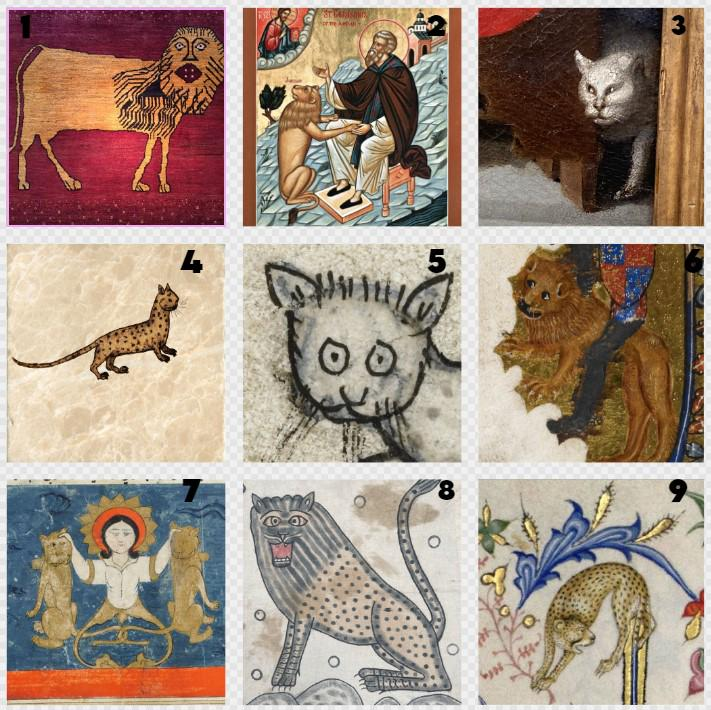
\includegraphics[width = .5\linewidth]{figs/MedievalCatIcebreaker.jpeg}
        \url{https://pollev.com/mykellorenbrinkerhoff821} or text/SMS mykellorenbrinkerhoff821 to 22333
    \end{center}
\end{frame}
\begin{frame}{Recap and Reflection}
    \begin{block}{Reflection}
        \begin{itemize}
            \item Spend $\thicksim$3 minutes reviewing your notes from last lecture and from R\&J ch. 2.
            \item Look for questions you have or clarifications you need. 
        \end{itemize}
    \end{block}
\end{frame}

%-----------------------------------------------------------
\section{More about the IPA}
%-----------------------------------------------------------

\begin{frame}{The International Phonetic Alphabet}
    \begin{itemize}
        \item A transcription system with the goal of describing the sounds found in all the world’s languages

        \item While the human vocal tract can produce an amazing array of sounds, the ones used in languages are more limited (~200)

        \item Any individual language has a much smaller number of sounds in its inventory (all the speech sounds used in that language)
        \begin{itemize}
            \item Rotokas (~11)
            \item !Xóõ (~122)
        \end{itemize}
    \end{itemize}
\end{frame}

\begin{frame}{The IPA Chart}
    \begin{center}
        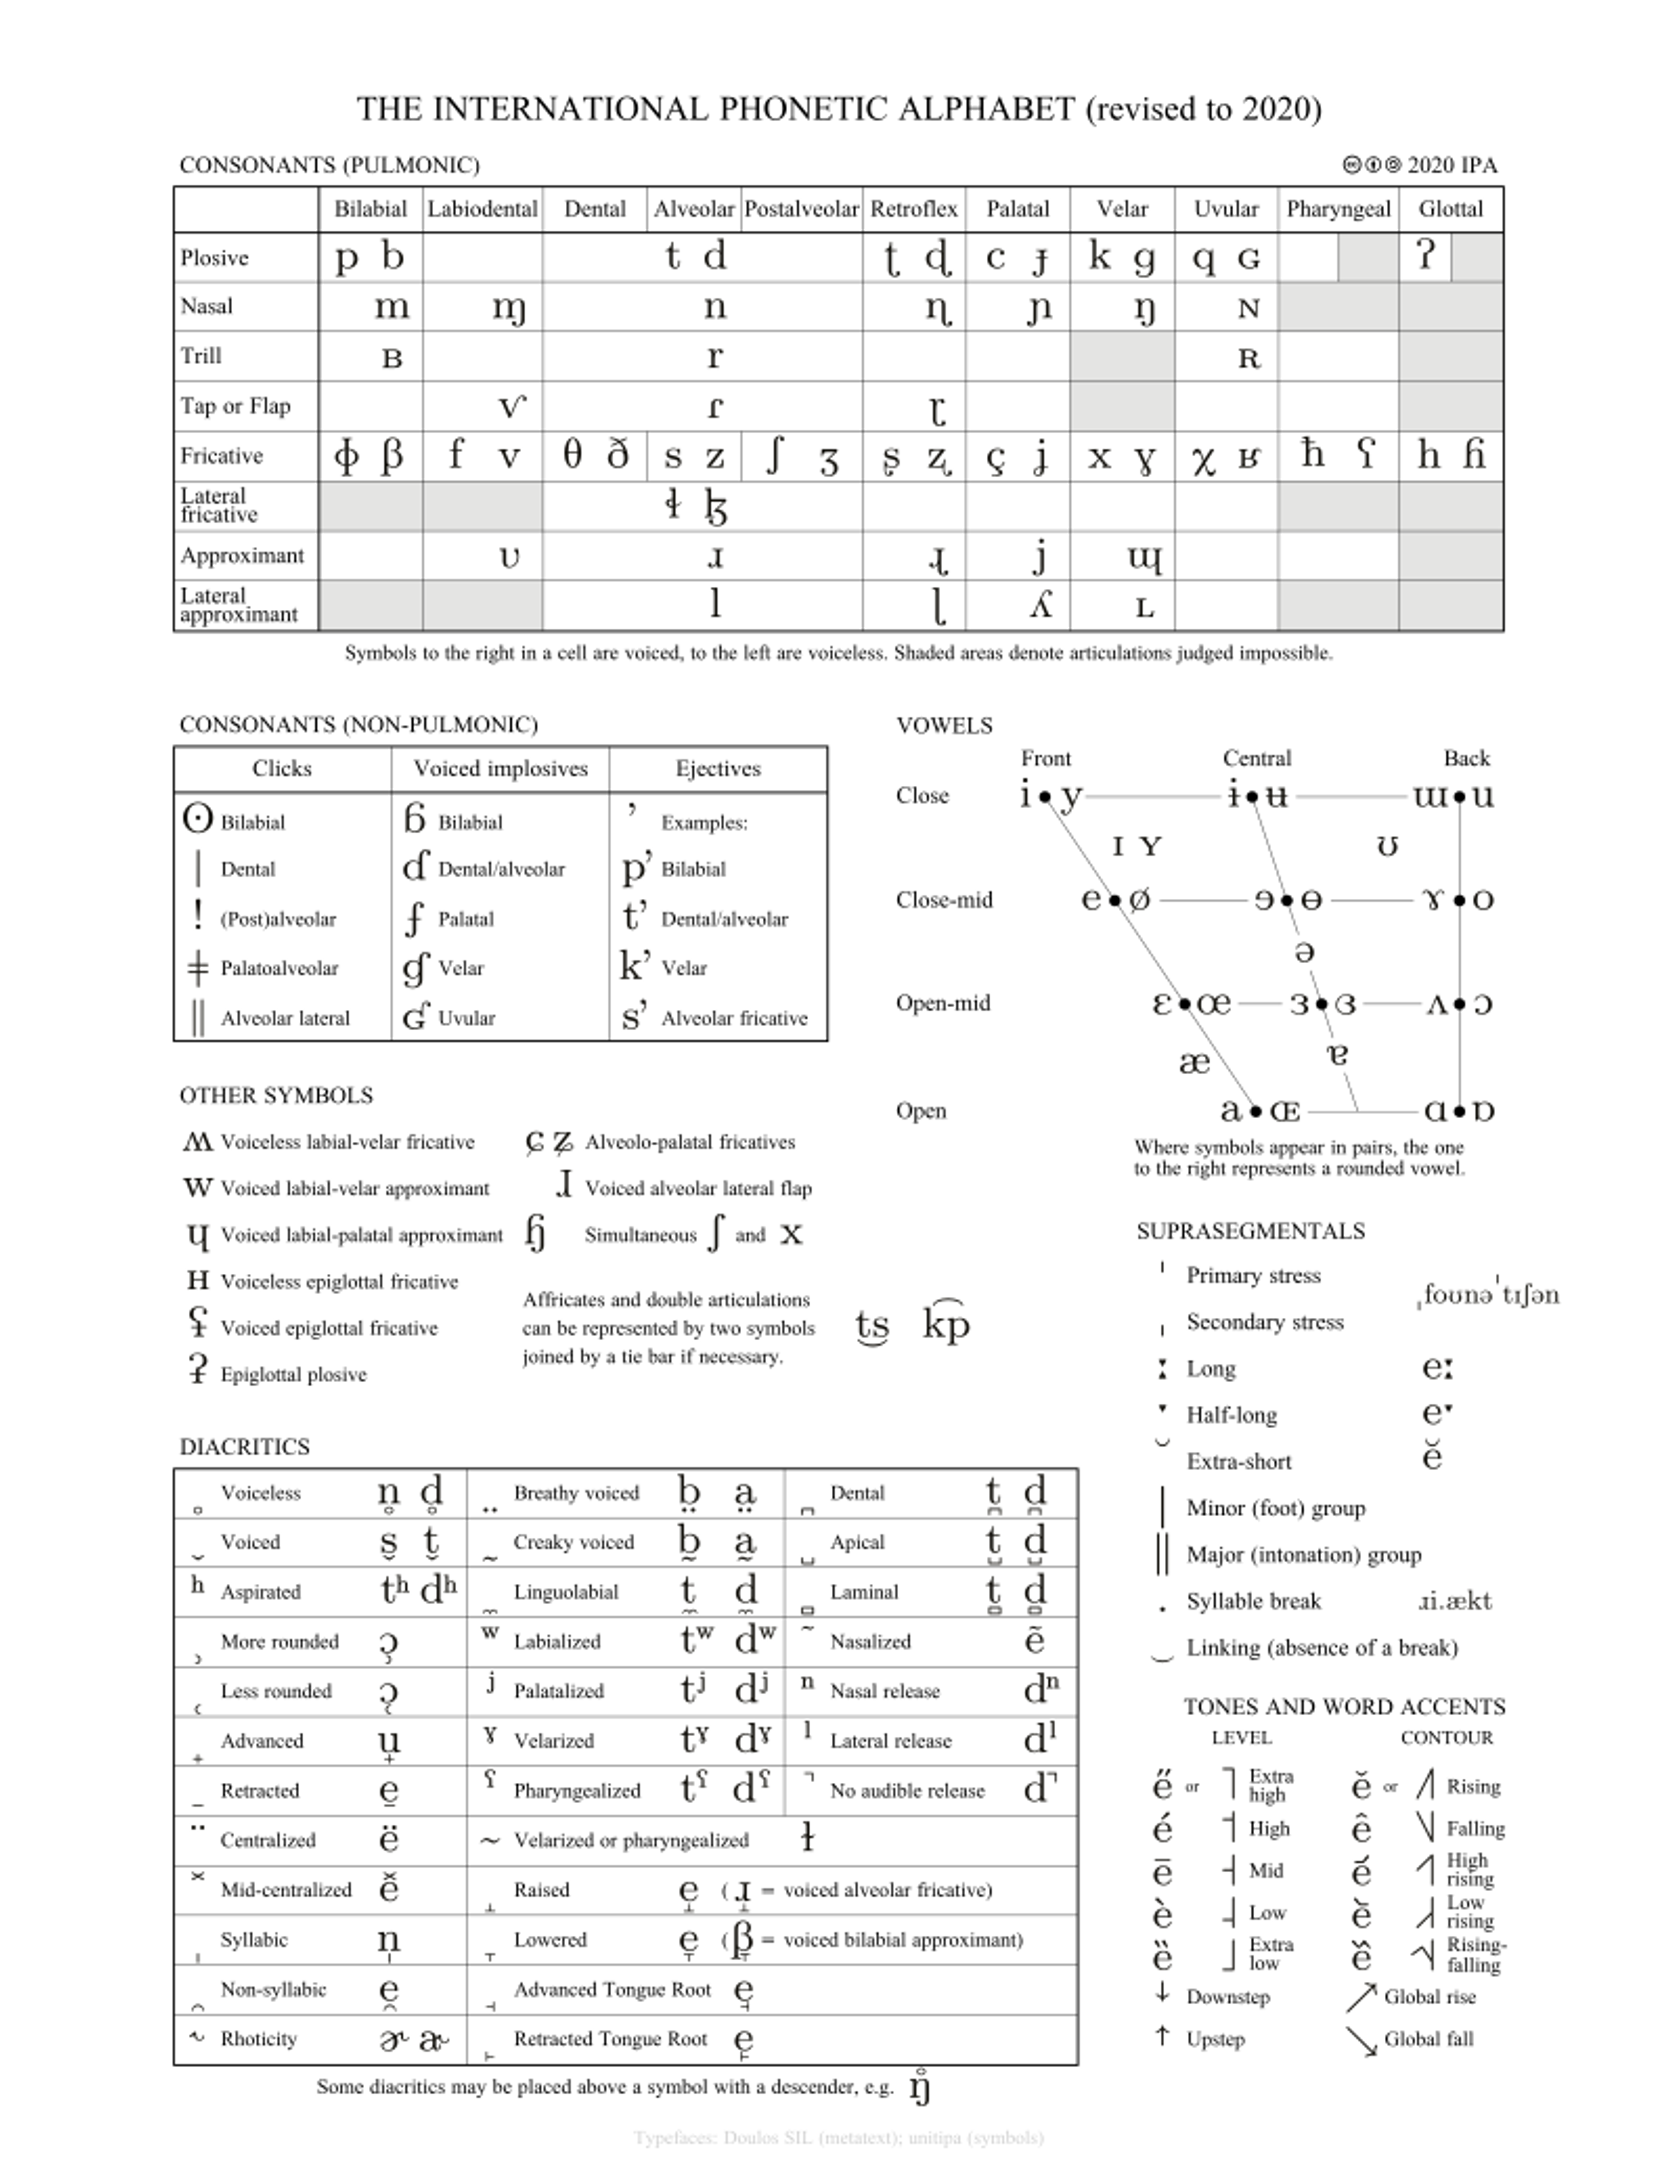
\includegraphics[width = .5\textwidth]{figs/IPAChart.png}
    \end{center}
\end{frame}

%-----------------------------------------------------------
\section{Speech articulators}
%-----------------------------------------------------------
\begin{frame}{Speech articulators}
    \begin{itemize}
        \item Most of these body parts have other essential functions--primarily breathing and eating
        \item They have been co-opted and adapted to speech through evolutionary processes
        \item In this class we're mostly talking about \textbf{descriptive articulation} (i.e., only a minimal examination of physiology and motor control)
    \end{itemize}
\end{frame}

\begin{frame}{Chimpanzee (\textit{Pan troglodytes}) vs. Human Vocal Tracts}
    \begin{center}
        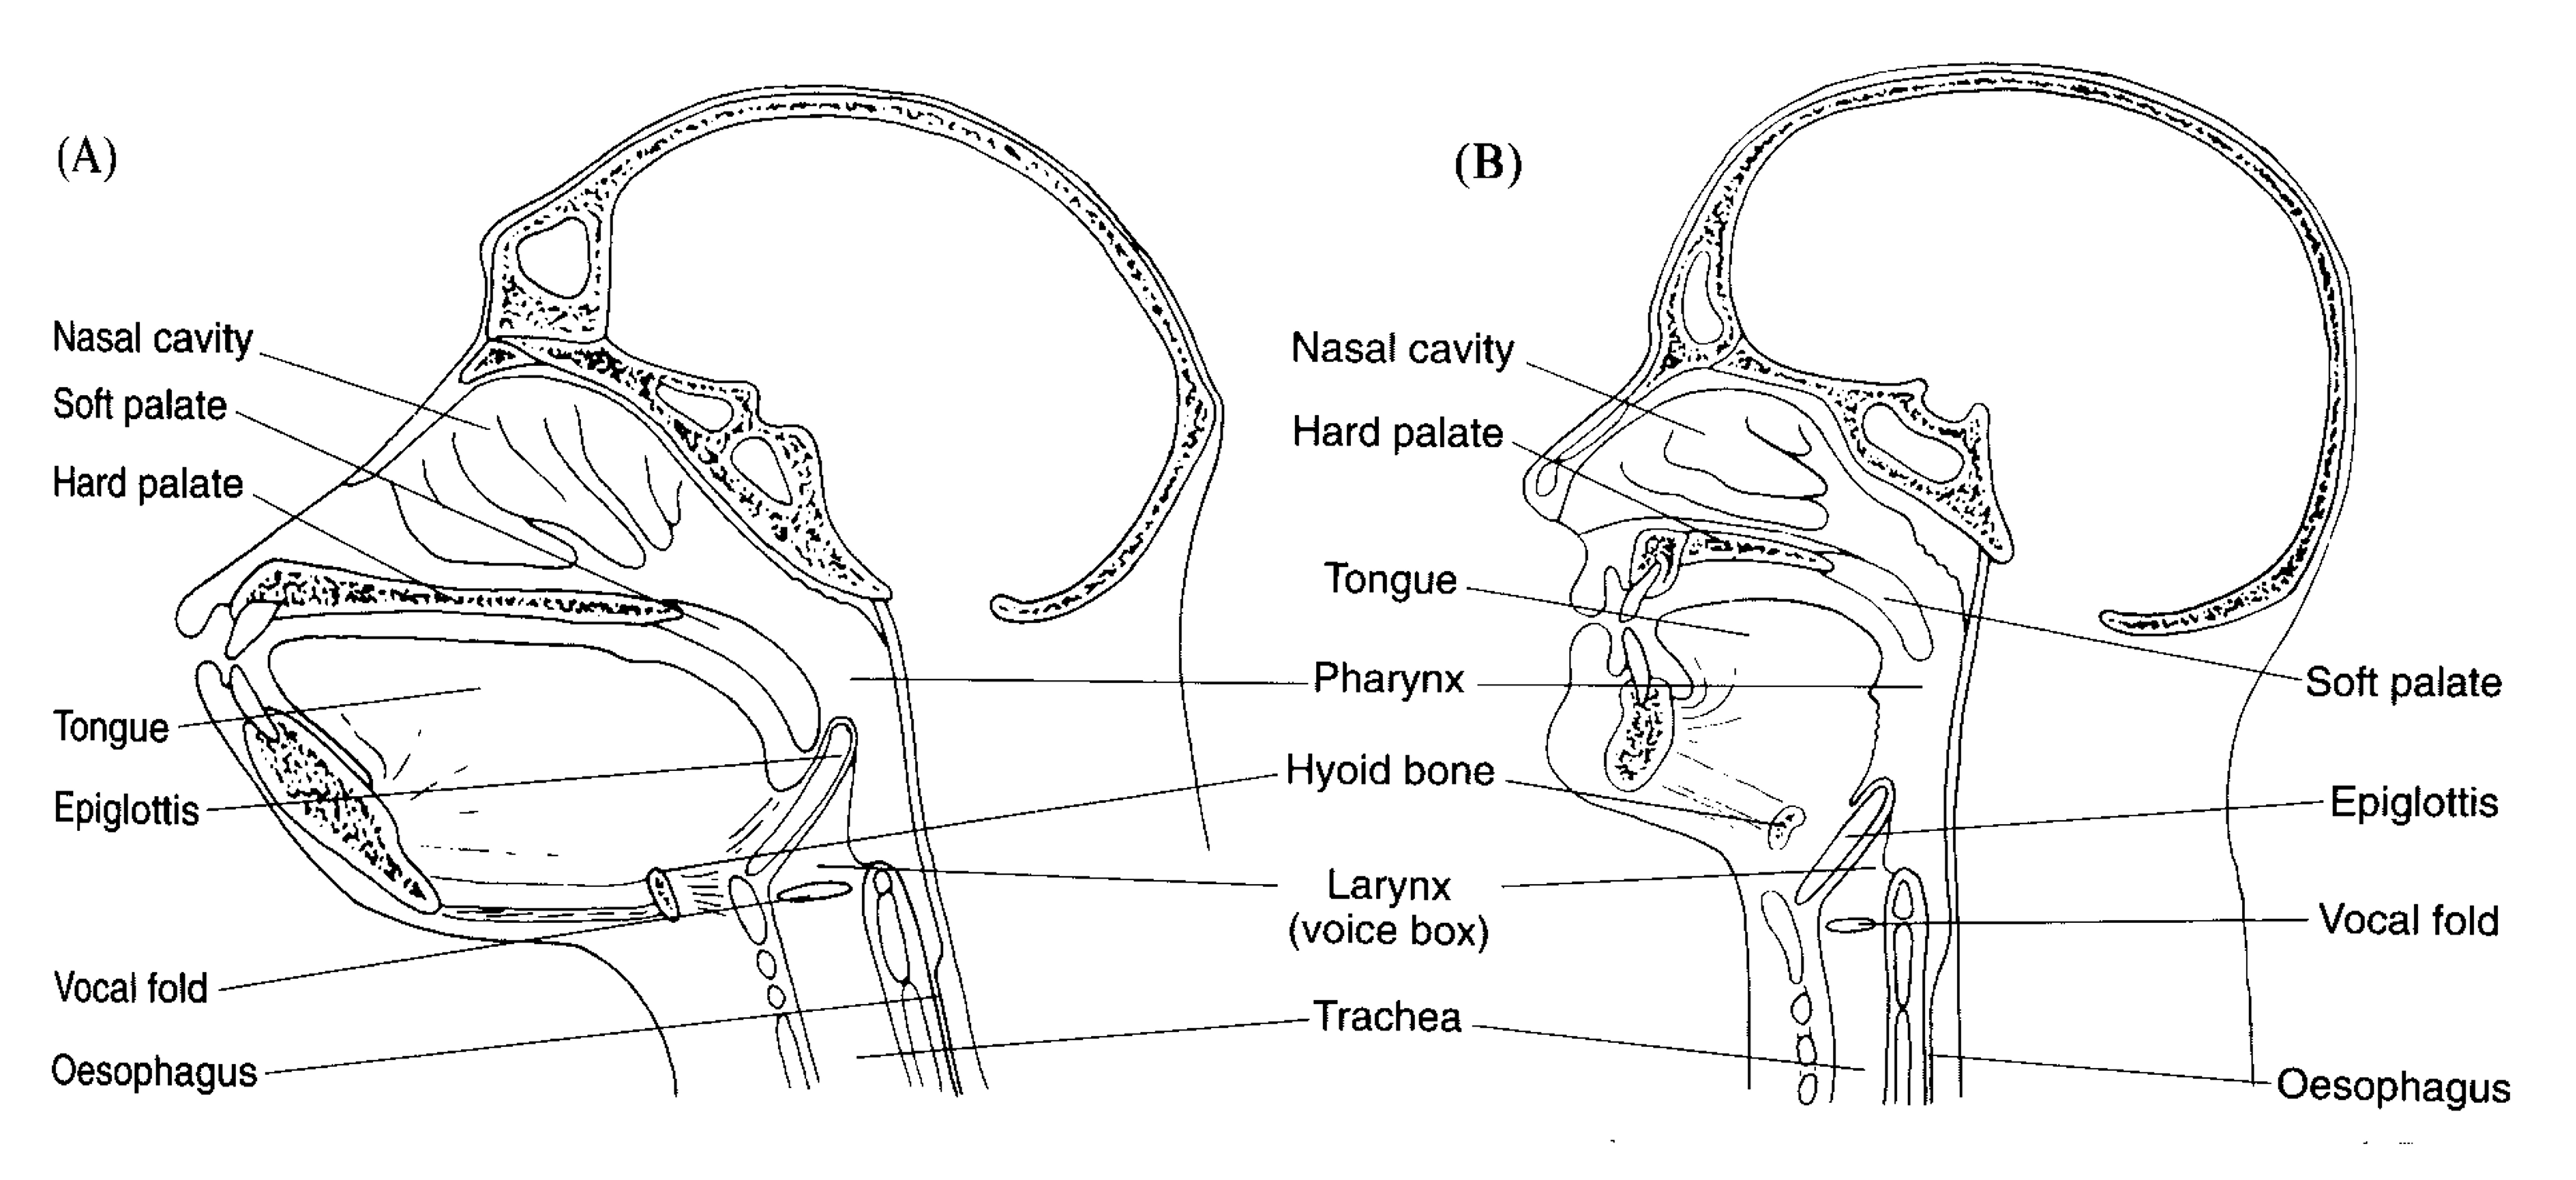
\includegraphics[width = \textwidth]{figs/ChimpanzeeVSHumanVT.png}
    \end{center}
\end{frame}

\begin{frame}{Human development}
    \begin{center}
        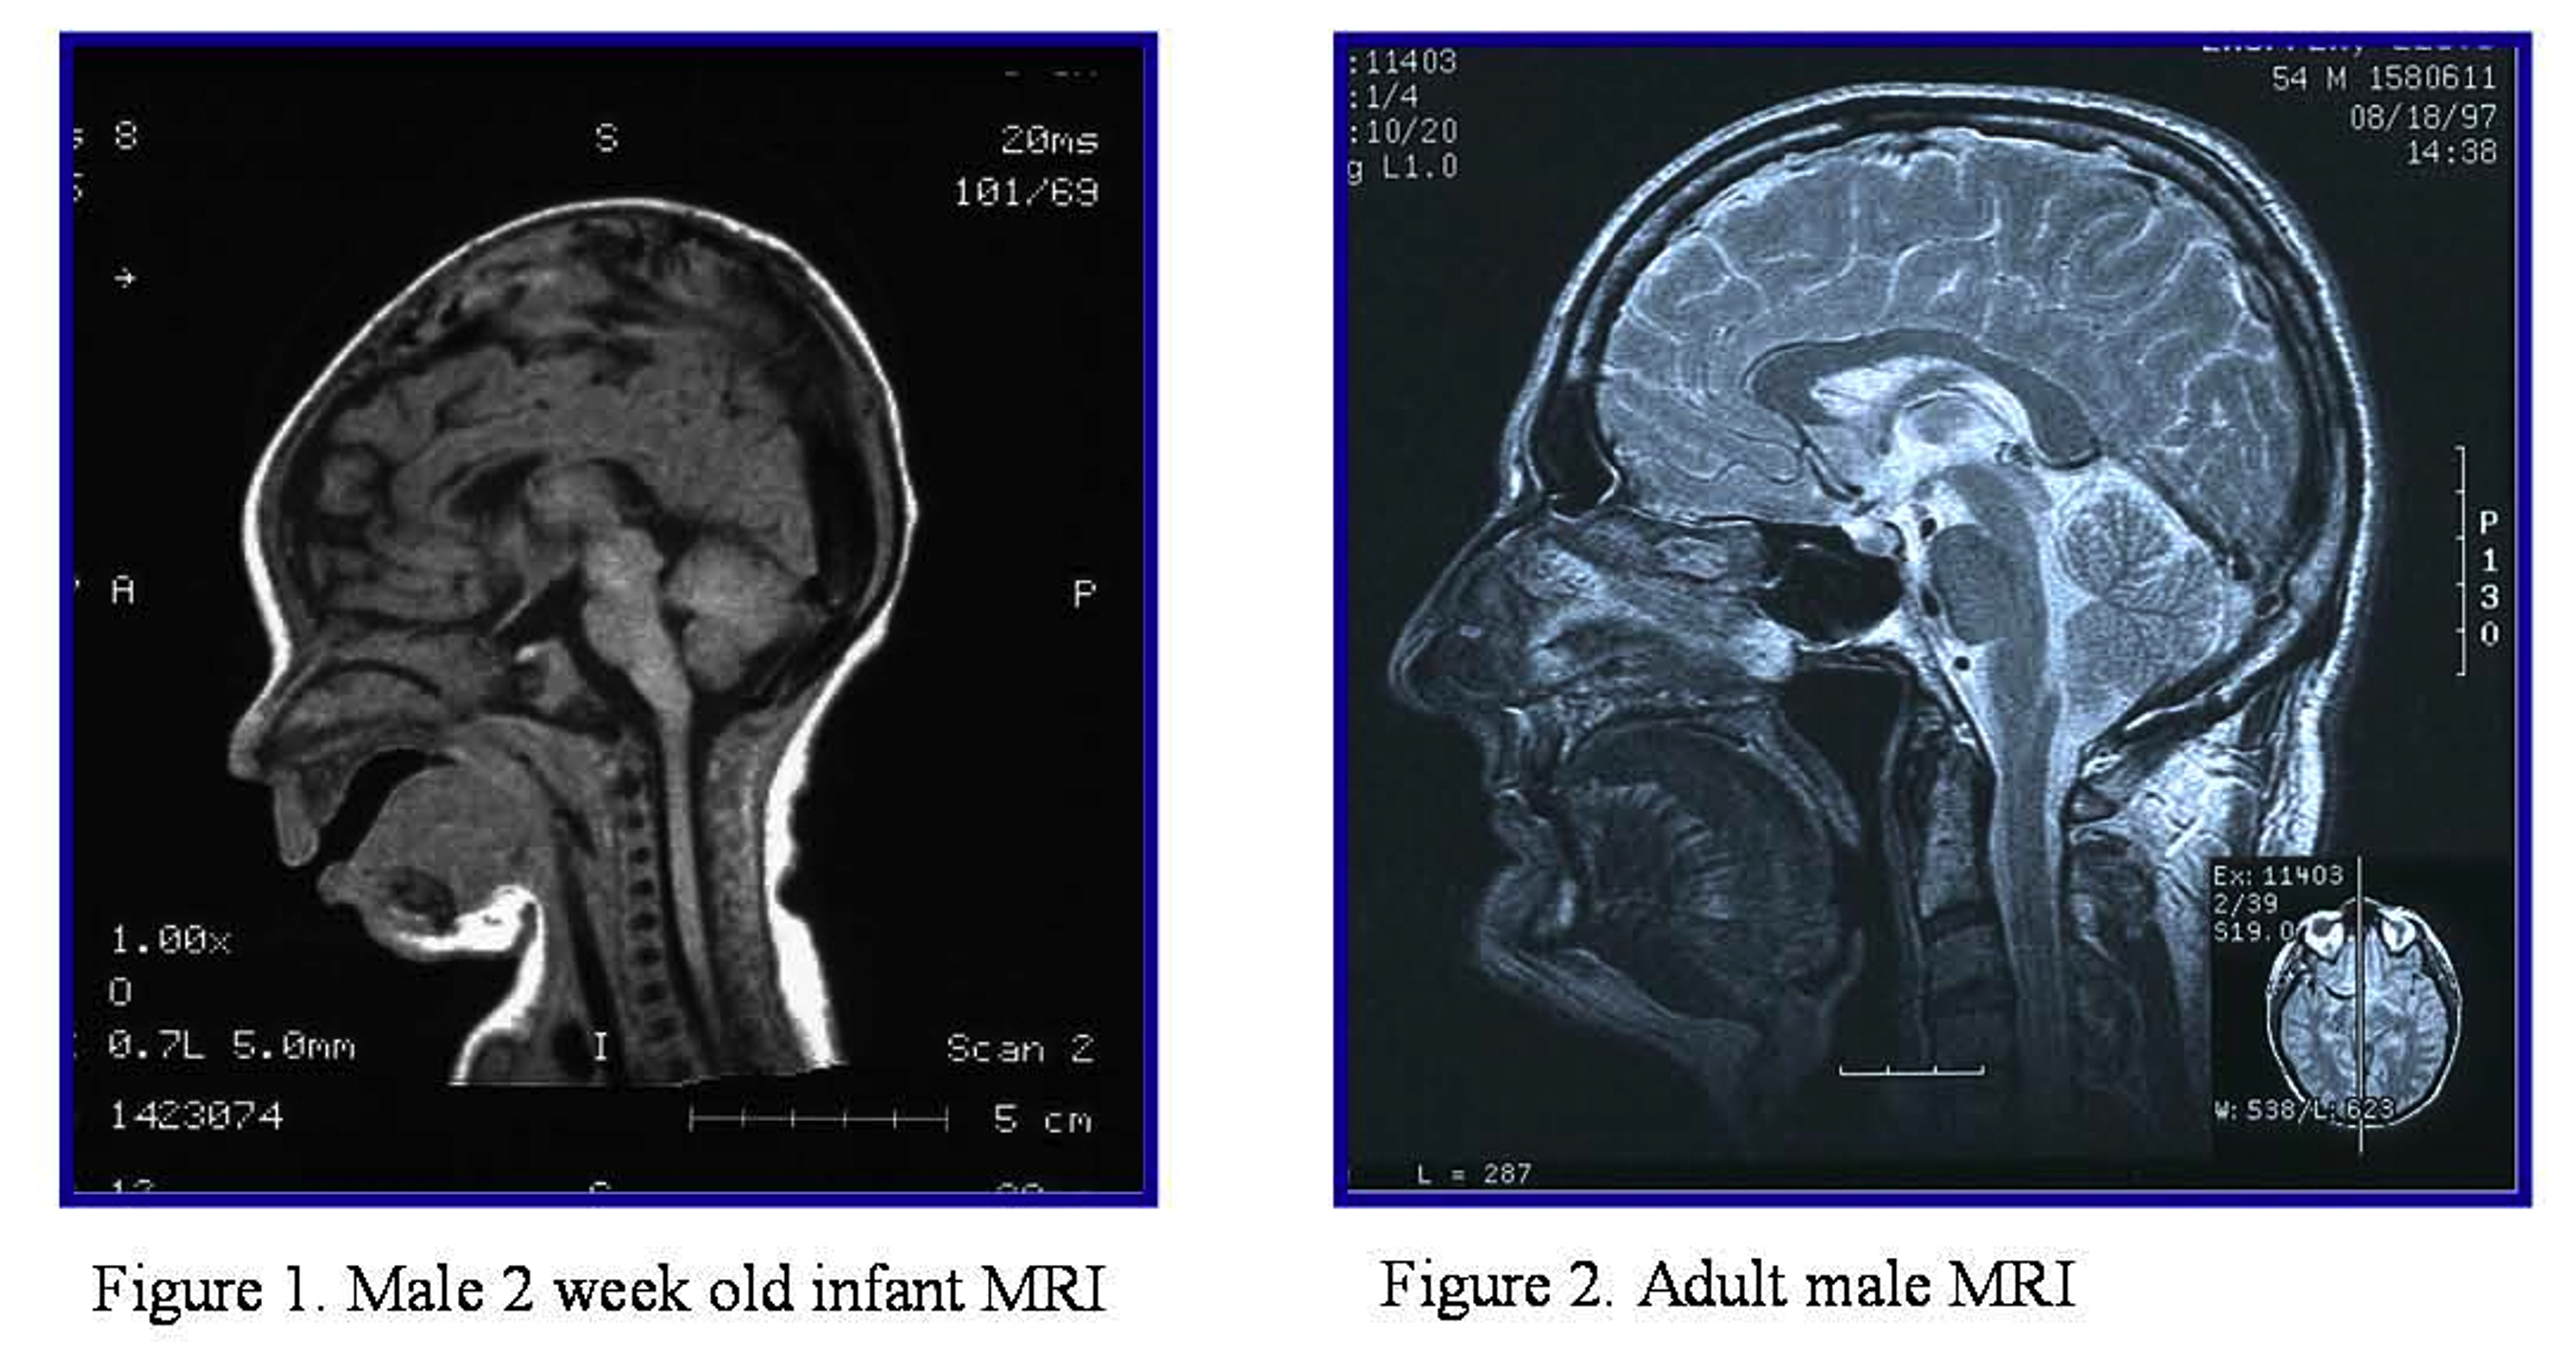
\includegraphics[width = \textwidth]{figs/HumanChildAdultMRI.png}
    \end{center}
\end{frame}

\begin{frame}{What does speech look like?}
    \begin{itemize}
        \item To begin, we need to understand the basic articulators for speech
        \item \href{https://youtu.be/DcNMCB-Gsn8?feature=shared}{Ken Steven's X-ray}
        \item \href{https://youtu.be/Wrbe5fH888k?feature=shared}{Vocal tract MRI during speech}
    \end{itemize}
\end{frame}

%-----------------------------------------------------------
\section*{Breathing}
%-----------------------------------------------------------

\begin{frame}{Breathing apparatus}
    \begin{itemize}
        \item The basic source of power in speech is the respiratory system pushing air out of the lungs
        \item In most instances, we superimpose speech on an outgoing breath
        \item Humans have considerable control over breathing, especially compared to other primates
    \end{itemize}
\end{frame}

\begin{frame}{Breathing}
    \begin{multicols}{2}
        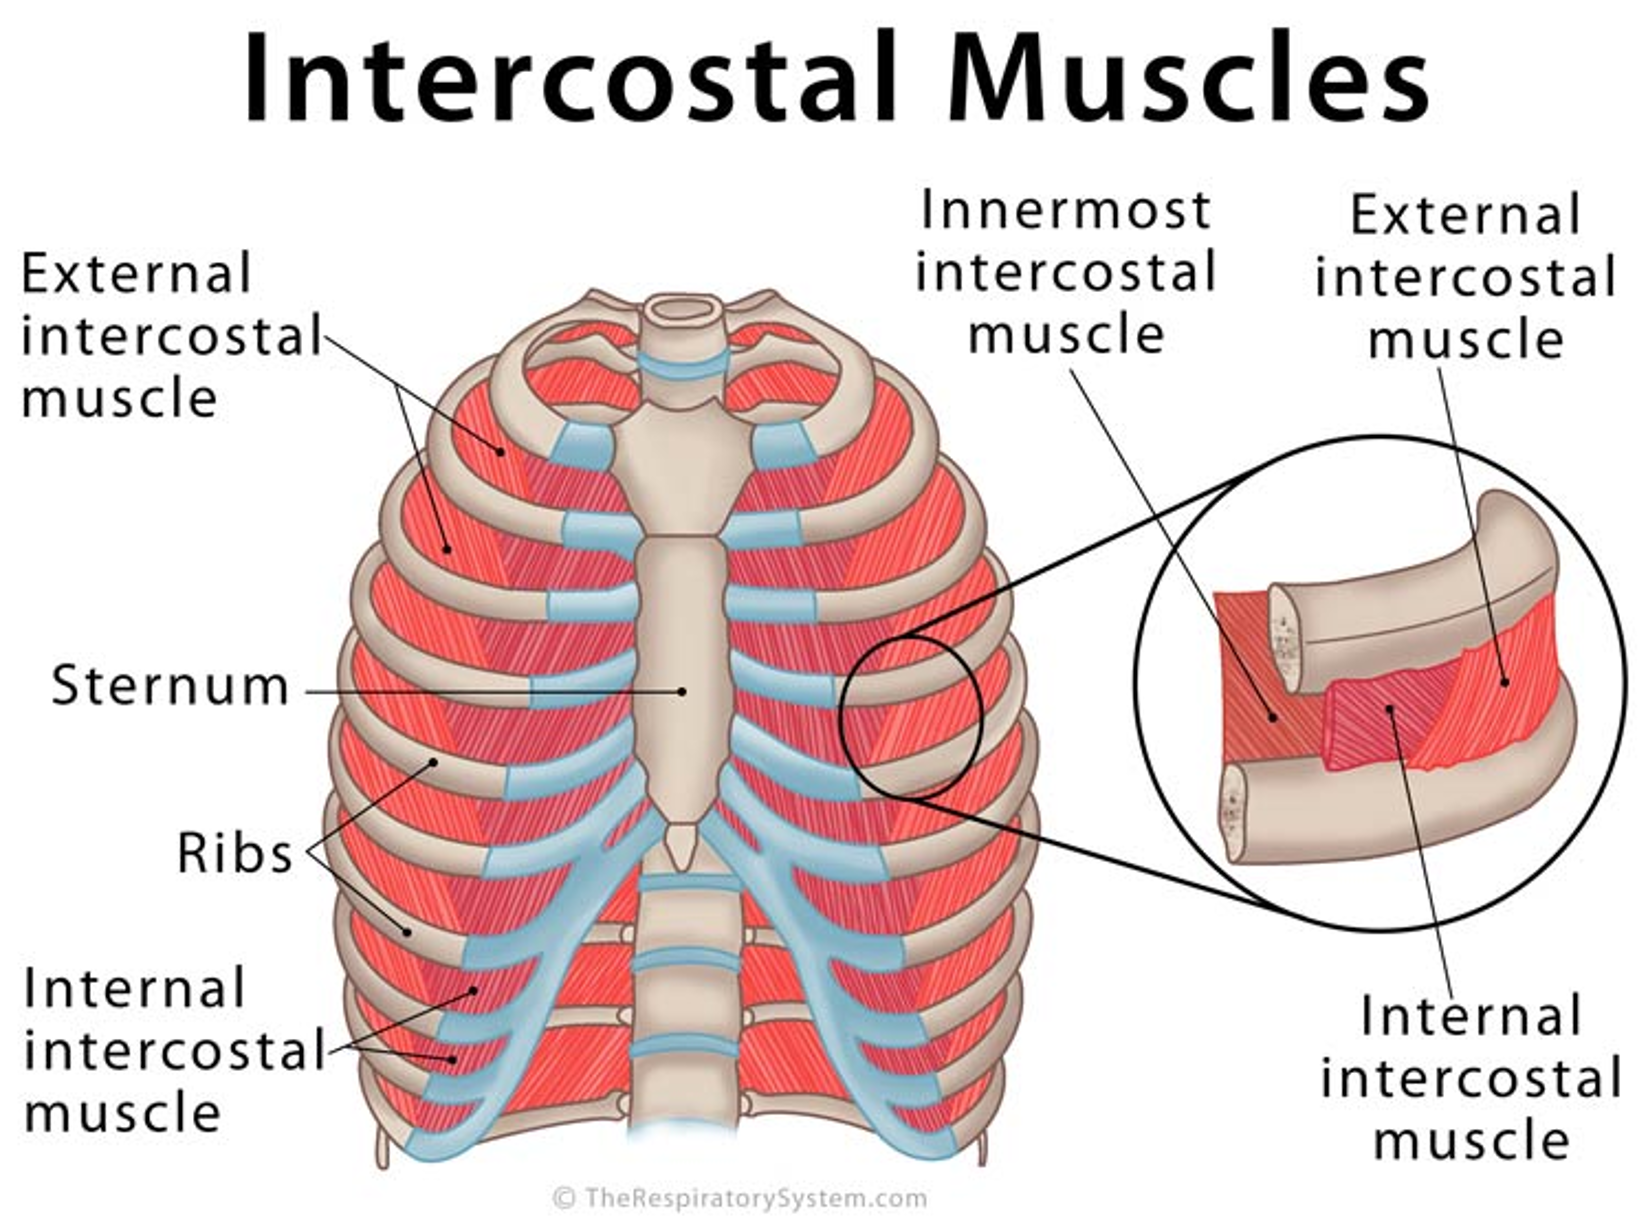
\includegraphics[width = \linewidth]{figs/IntercostalMuscles.png}
        \columnbreak
        \begin{itemize}
            \item \textbf{Inhalation:} the ribs are pulled up by the external intercostal muscles
            \item \textbf{Exhalation:} rib cage is deflated by pulling the ribs down by the internal intercostals
            \item Exhalation is a more passive activity in during \textbf{tidal breathing}—elastic tension on the ribs naturally compresses them
        \end{itemize}
    \end{multicols}
\end{frame}

\begin{frame}{Breathing for staying alive vs. speech}
    \begin{itemize}
        \item Both an active and passive process
        \item \textbf{Respiration} is breathing to stay alive. It’s mostly unconscious, controlled by the brainstem—regulated primarily by blood pH
        \item \textbf{Speech breathing} is a very different story 
    \end{itemize}
\end{frame}

\begin{frame}{Speech breathing}
    \begin{itemize}
        \item Higher level motor control regions interact with the brainstem to control breathing 
        \item Inhalations timed for major phrasal/sentence boundaries depending on overall utterance length 
        \item Depth of inhalation and speed of exhalation controlled to utter the desired amount of speech per breath cycle 
        \item A learned behavior—notice that children and very excited people often get out of breath while talking 
    \end{itemize}
\end{frame}

\begin{frame}{Speech breathing}
    \begin{center}
        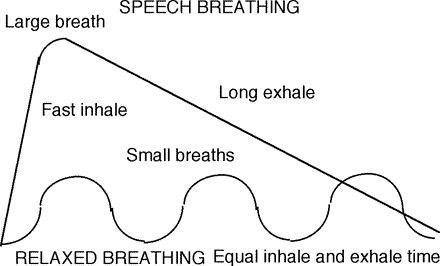
\includegraphics[width = .75\textwidth]{figs/SpeechBreathing.png}
    \end{center}
\end{frame}

\begin{frame}{A small note}
    \begin{itemize}
        \item We will be coming back to the physics in a few weeks. 
    \end{itemize}
\end{frame}

%-----------------------------------------------------------
\section*{Larynx}
%-----------------------------------------------------------

\begin{frame}{The larynx and glottis}
    \begin{itemize}
        \item Reminder: the \textbf{larynx} is the entire structure that holds the vocal folds (plural is larynges)
        \begin{itemize}
            \item Can also move up and down as a kind of articulator (e.g., ejective and implosive consonants)
            \item Consonants made here are \textbf{laryngeal}
        \end{itemize}
        \item Consonants articulated by opening and closing the vocal folds are \textbf{glottal}
        \begin{itemize}
            \item Only if the opening or closing of the glottis the primary articulation (e.g., not just voicing)
        \end{itemize}
        \item There's lots of confusion in the field between the terms
    \end{itemize}
\end{frame}

\begin{frame}{The Larynx}
    \begin{center}
        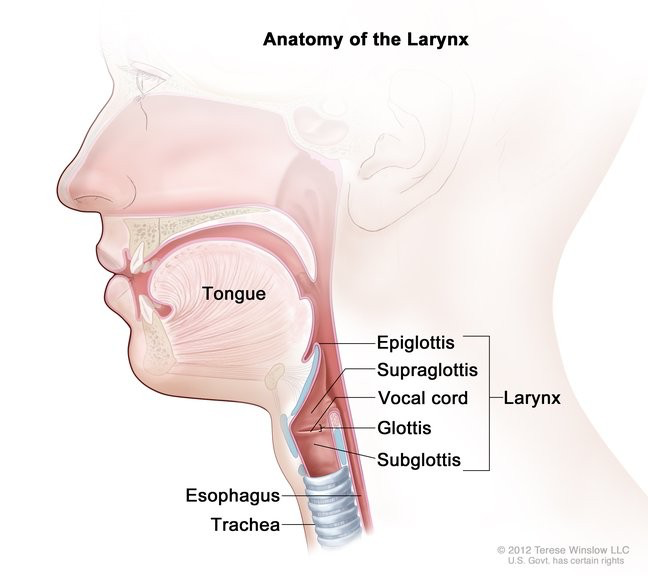
\includegraphics[width = 0.75\textwidth]{figs/AnatamyLarynx.png}
    \end{center}
\end{frame}

\begin{frame}{Major structures of the larynx}
    \begin{center}
        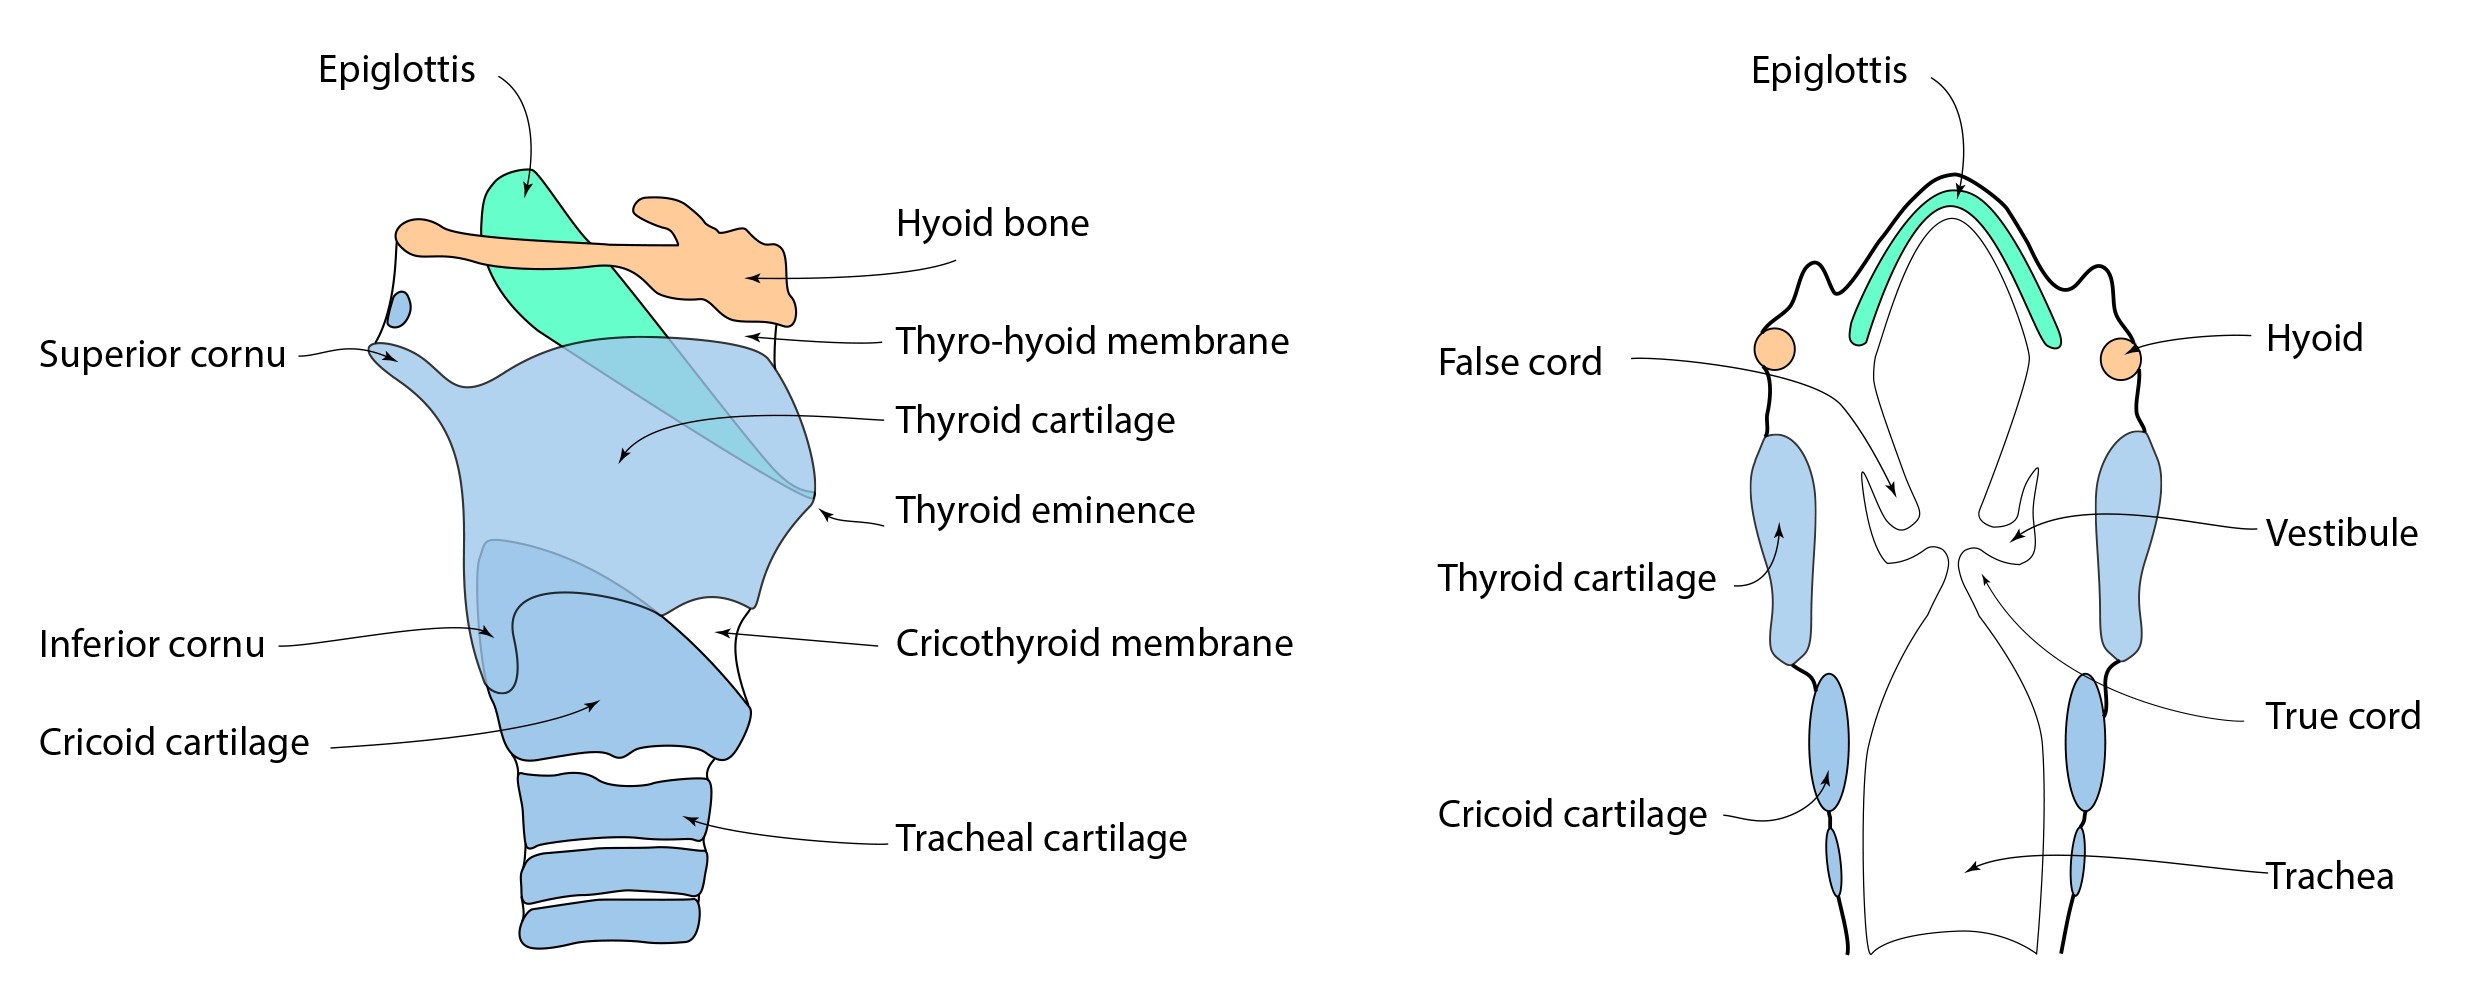
\includegraphics[width = \textwidth]{figs/LarynxStructures_Major.png}
    \end{center}
\end{frame}

\begin{frame}
    \frametitle{How the larynx works}
    \begin{multicols}{2}
        
    \begin{itemize}
        \item The triangular-shaped \textbf{arytenoid cartilages} sit on the upper back of the \textbf{crycoid cartilage}
        \item They \textbf{rotate} and \textbf{slide} to \textit{abduct} (move apart) and \textit{adduct} (bring together) the vocal folds
    \end{itemize}

    \columnbreak
    
    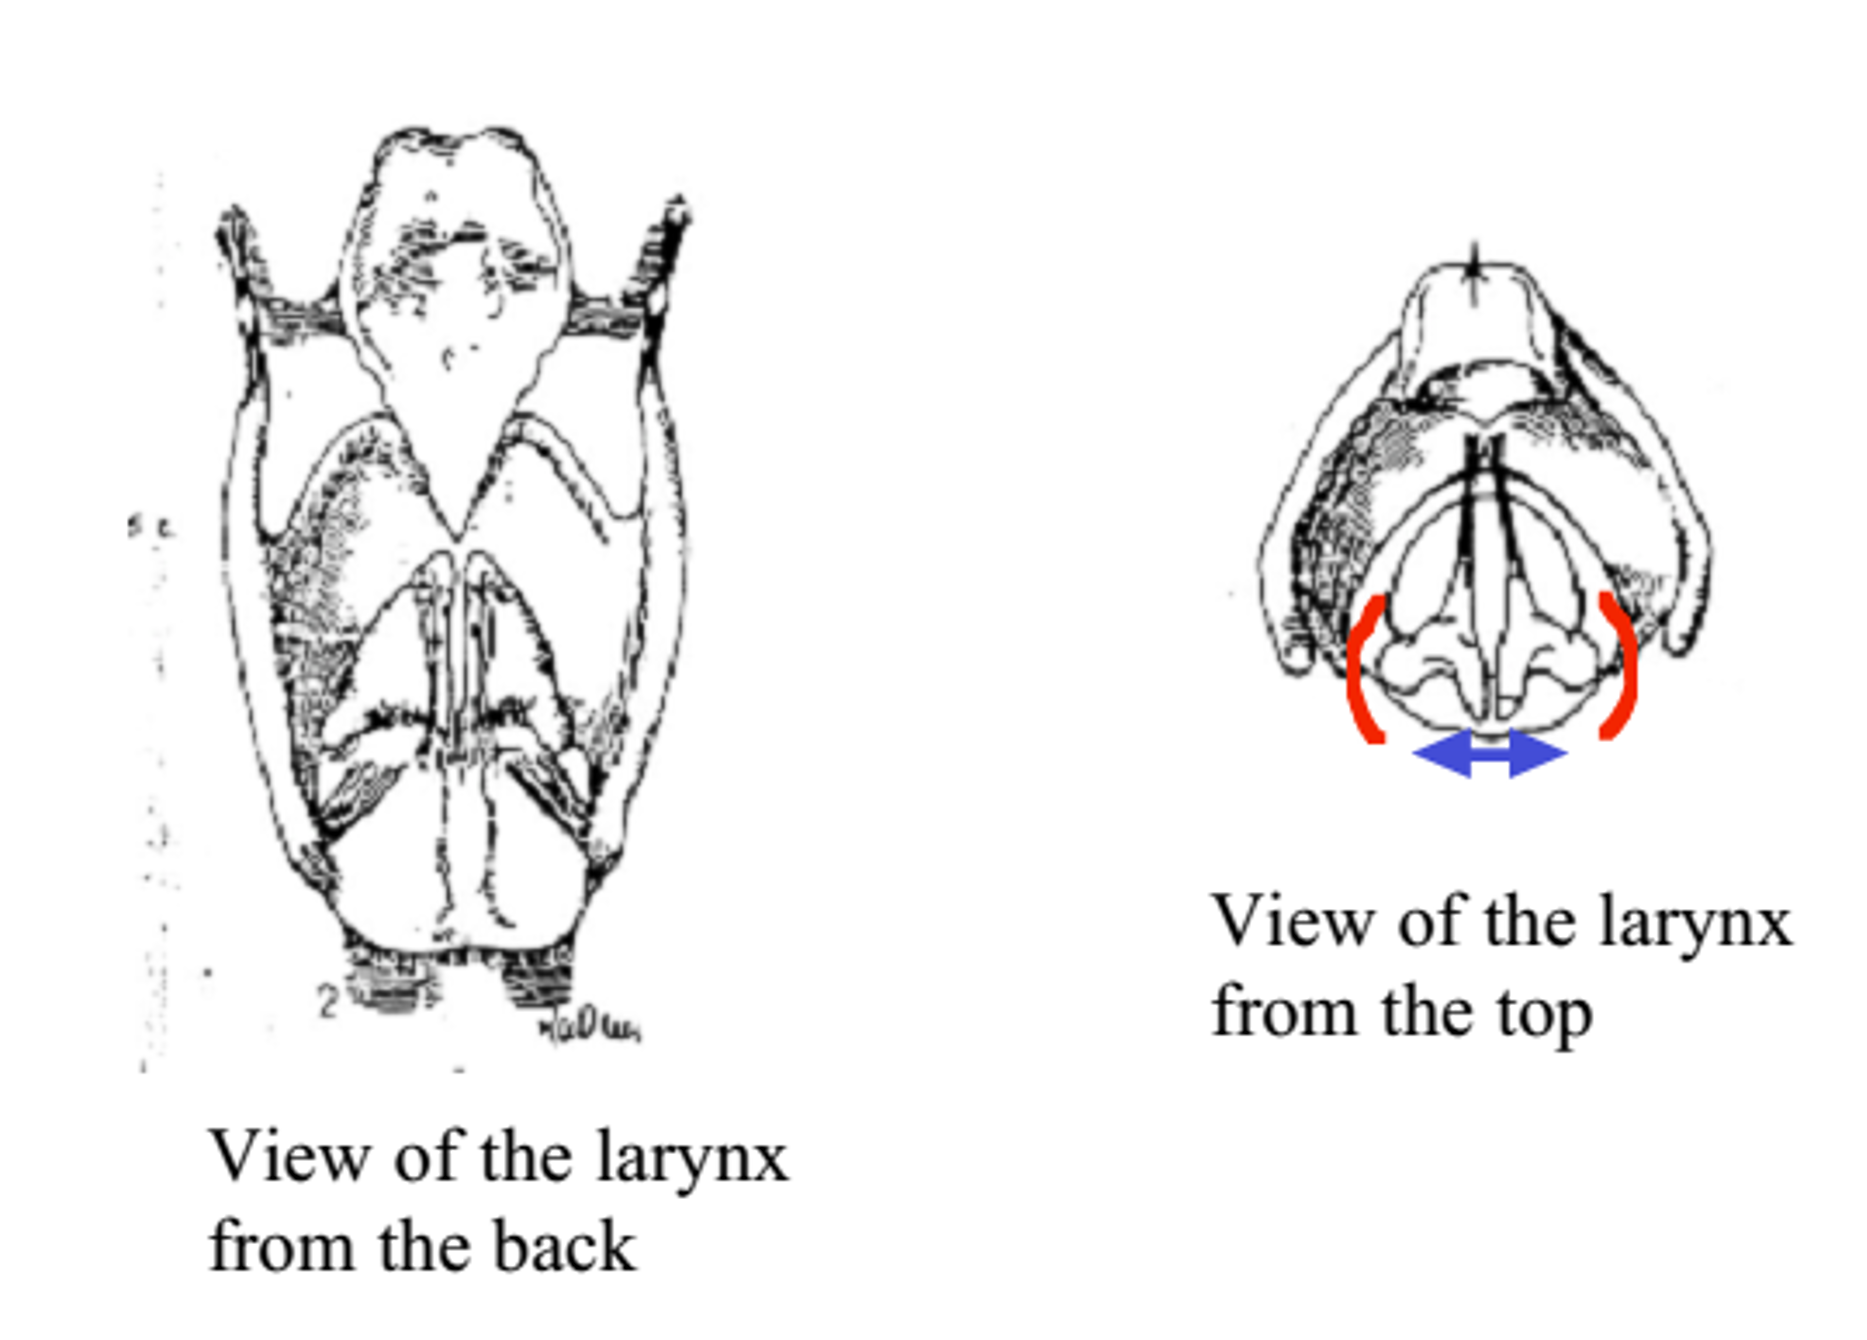
\includegraphics[width = \linewidth]{figs/Cartilages.png}

    \end{multicols}
\end{frame}

\begin{frame}{How the larynx works}
    \begin{multicols}{2}

        \begin{itemize}
            \item The length of the vocal folds is correlated with the angle between the thyroid cartilage and the cricoid cartilage
            \item When the thyroid is tilted \textcolor{green}{forward} the vocal folds are longer and thinner
            \item When the thyroid is tilted \textcolor{red}{back} the vocal folds are shorter and thus thicker and vibrate at a lower rate
        \end{itemize}

        \columnbreak

        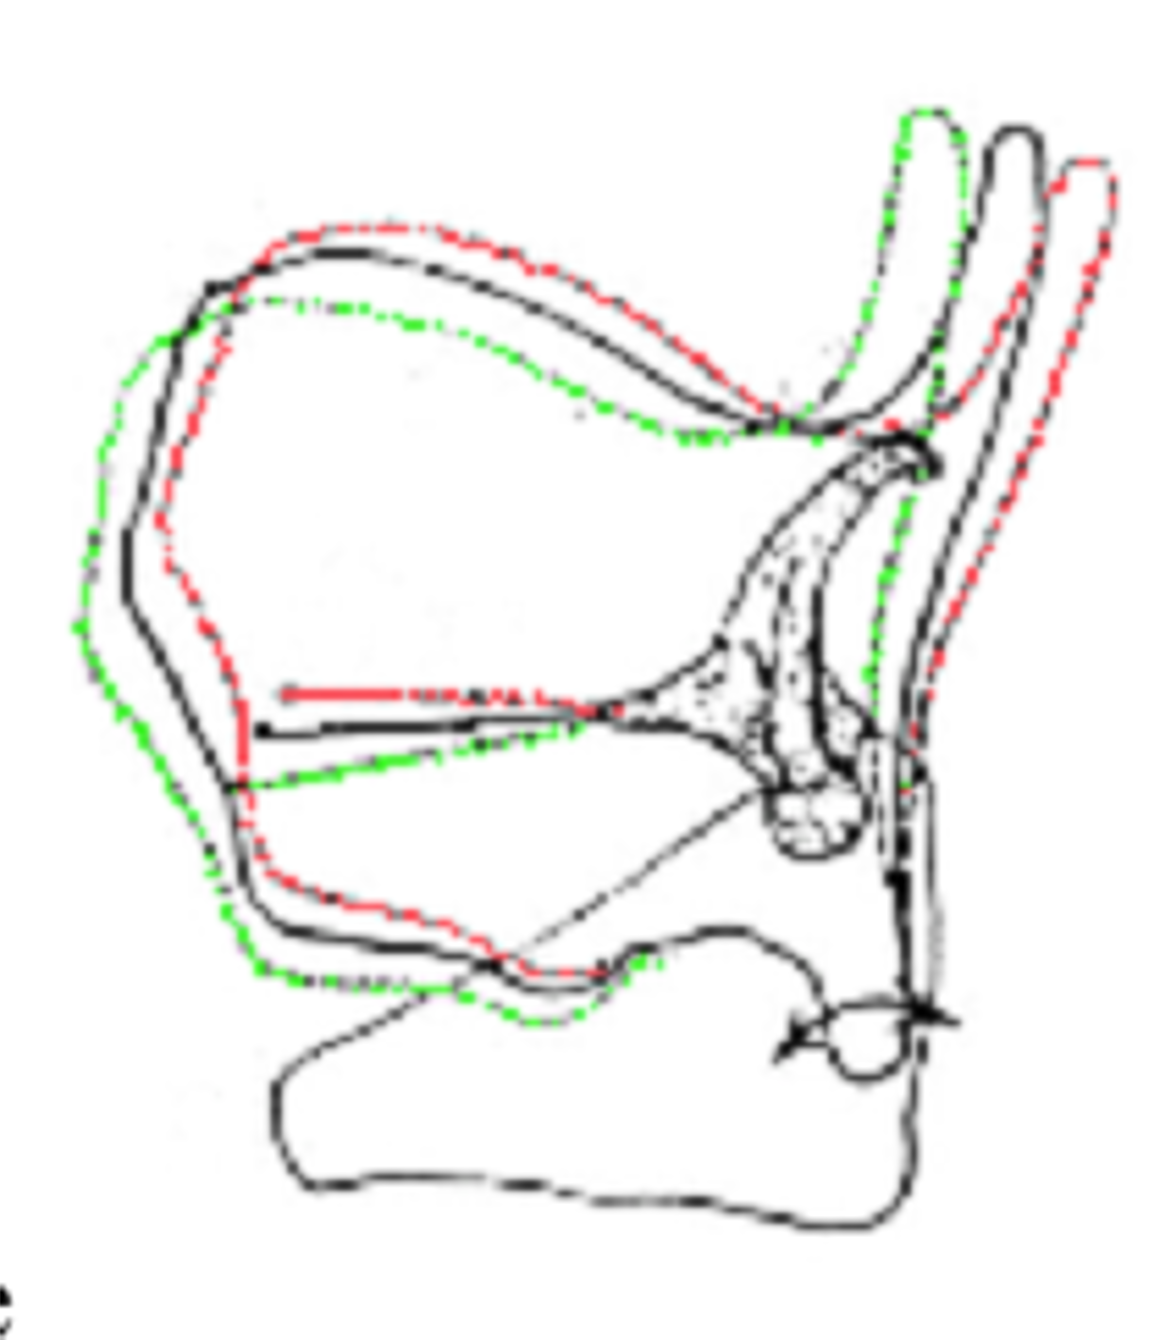
\includegraphics[width = \linewidth]{figs/LaryngealTilt.png}

    \end{multicols}
\end{frame}

\begin{frame}{Muscle in the larynx}
    \begin{multicols}{2}
        \begin{itemize}
            \item The main muscle in the larynx that controls the pitch of the voice is the \textbf{cricothyroid muscle}
        \end{itemize}
        \columnbreak
        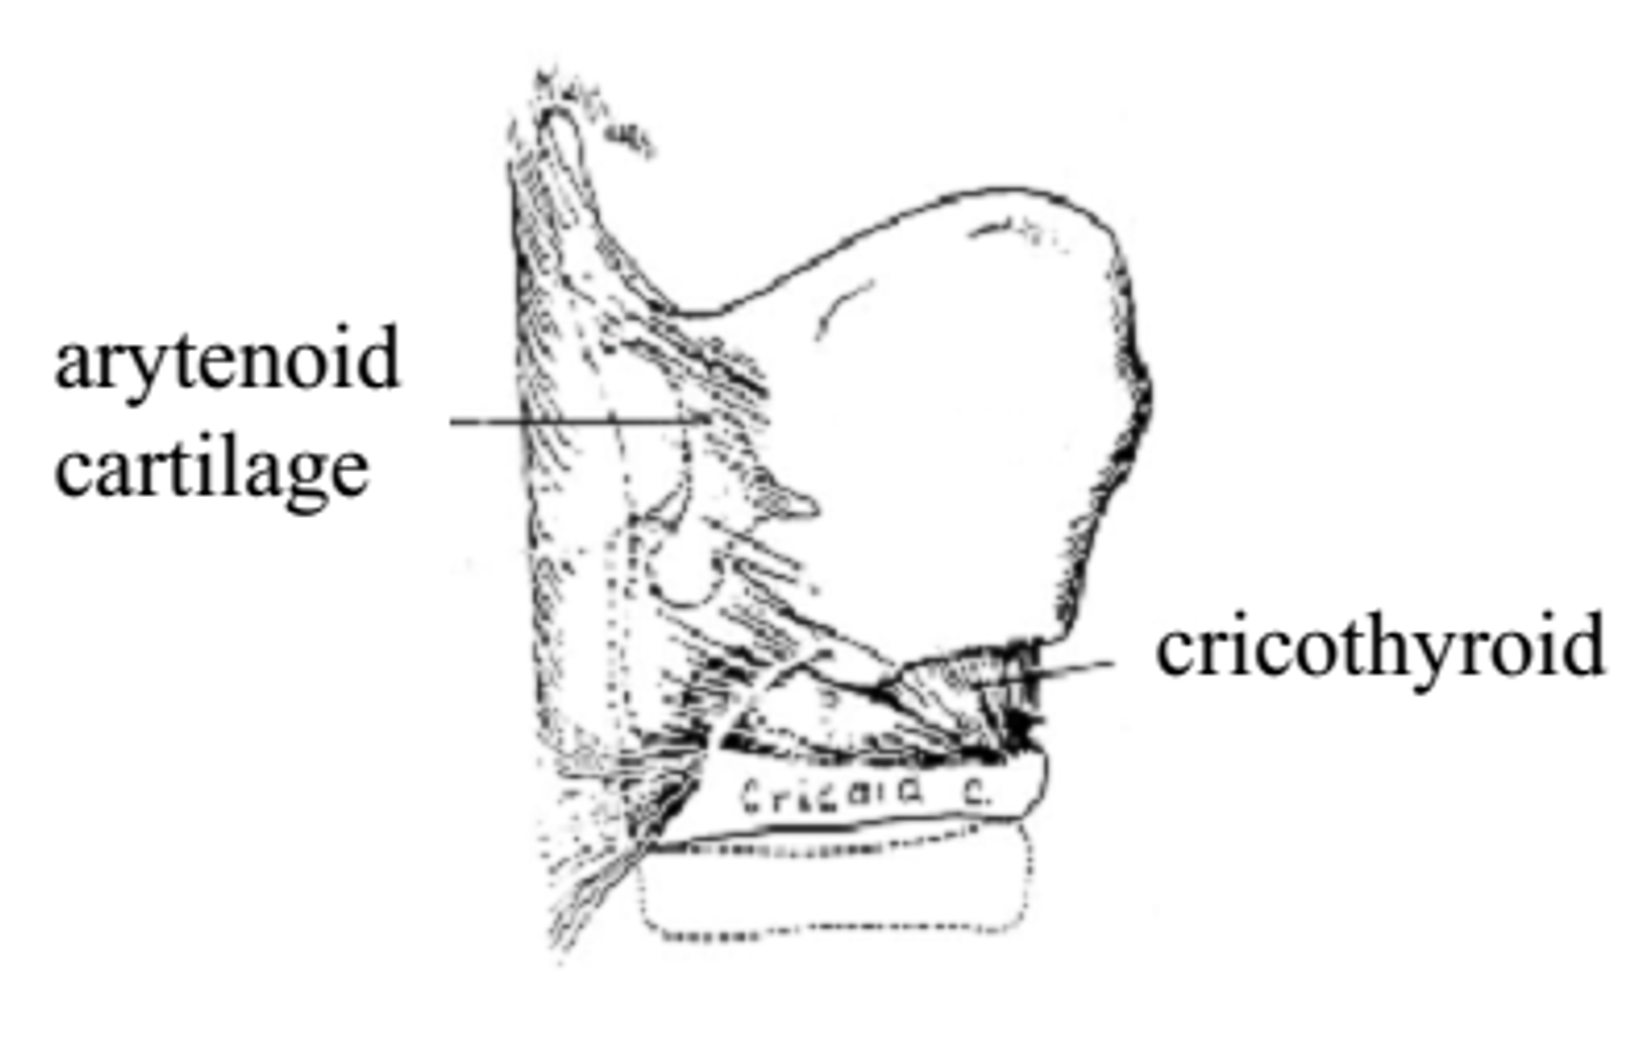
\includegraphics[width = \linewidth]{figs/Cricothyroid.png}
    \end{multicols}
\end{frame}

%-----------------------------------------------------------
\section*{Vocal folds}
%-----------------------------------------------------------

\begin{frame}{The vocal folds}
    \begin{itemize}
        \item Tissue folds crucial to voicing
        \item Hormone changes at puberty stimulate enlarging in adolescents (roughly, more testosterone ≈ larger vocal folds)
        \begin{itemize}
            \item Range from 12.5mm to 25mm in length, 3-5mm thick
            \item The larynx also lowers for all people, with more lowering corresponding to (roughly) more testosterone
        \end{itemize}
        \item More massive folds result in slower vibration (= lower pitch, on average)
        \item Most research has been with \textit{WEIRD}\footnote{Term coined in 2010 by Henrich, Heine, and Norenzayn to describe how 96\% of psychological samples come from \textit{W}estern, \textit{E}ducated, \textit{I}ndustrialized, \textit{R}ich, and \textit{D}emocratic societies.} societies, so take a lot of this with grain of salt (maybe even a pound *shrug*)
    \end{itemize}
\end{frame}

\begin{frame}{Vocal folds during speech}
    \begin{itemize}
        \item Higher pressure air resulting from lung compression flows to the lower pressure (usually atmospheric) in the oral cavity
        \item We think of ``pushing'' air through the vocal tract, but it's better to think about air flowing from higher to lower pressure (i.e., the Bernoulli effect)
        \item The lungs create pressure greater than atmospheric pressure when they compress
        \item Airflow passing through the adducted (= pulled together) vocal folds results in \textit{voicing}
    \end{itemize}
\end{frame}

\begin{frame}{The vocal folds during speech}
    \begin{multicols}{2}
        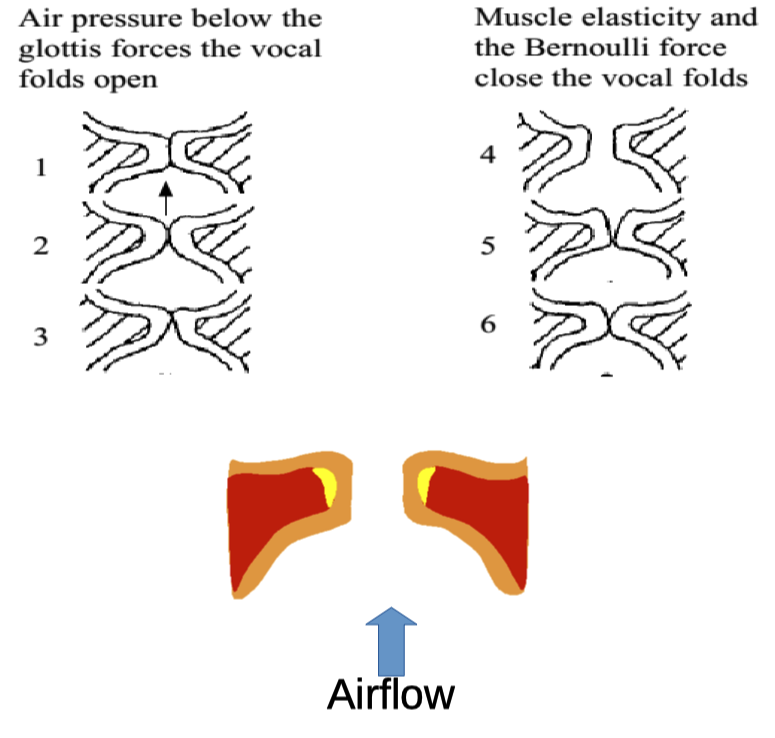
\includegraphics[width = \linewidth]{figs/Phonation.png}

        \columnbreak

        \begin{itemize}
        \item \textbf{Phonation}: setting the vocal folds into vibration
        \item Broader definition: any active modification of airflow by the larynx (This make my research really difficult)
        \item Also called: \textbf{voice}, \textbf{voicing}
        \item Videos:
        \begin{itemize}
            \item \href{https://voice.weill.cornell.edu/voice-evaluation/normal-voice-function}{Movies of vocal folds in action}
            \item \href{https://youtu.be/wR41CRbIjV4?feature=shared}{Synthesis}
            \item \href{https://youtu.be/UsFtDdd3emE?feature=shared&t=12}{Mucosal wave}
        \end{itemize}
    \end{itemize}
    \end{multicols}
\end{frame}

%-----------------------------------------------------------
\section*{Break}
%-----------------------------------------------------------

\begin{frame}{Break Time!}
    \begin{center}
        \Huge 10 minute break \\ (stretch, grab a drink, etc.)
    \end{center}
\end{frame}

%-----------------------------------------------------------
\section*{Articulators}
%-----------------------------------------------------------

\begin{frame}{Articulators}
    \begin{itemize}
        \item All articulators come in two flavors: 
        \begin{itemize}
            \item \textbf{Active articulators} move to produce a sound
            \item \textbf{Passive articulators} are static landmarks
        \end{itemize}
        \item Active articulators always move towards passive ones
        \item \textbf{Constrictions} pretty much all sounds are made by constrictions — two articulators actively narrowing some point (or points) of the vocal tract
        \begin{itemize}
            \item This means that we could potentially just use the physics of tubes to explain what occurs acoustically. 
            \item More to come in a few weeks
        \end{itemize}
    \end{itemize}
\end{frame}

\begin{frame}{The tongue}
    \begin{multicols}{2}

        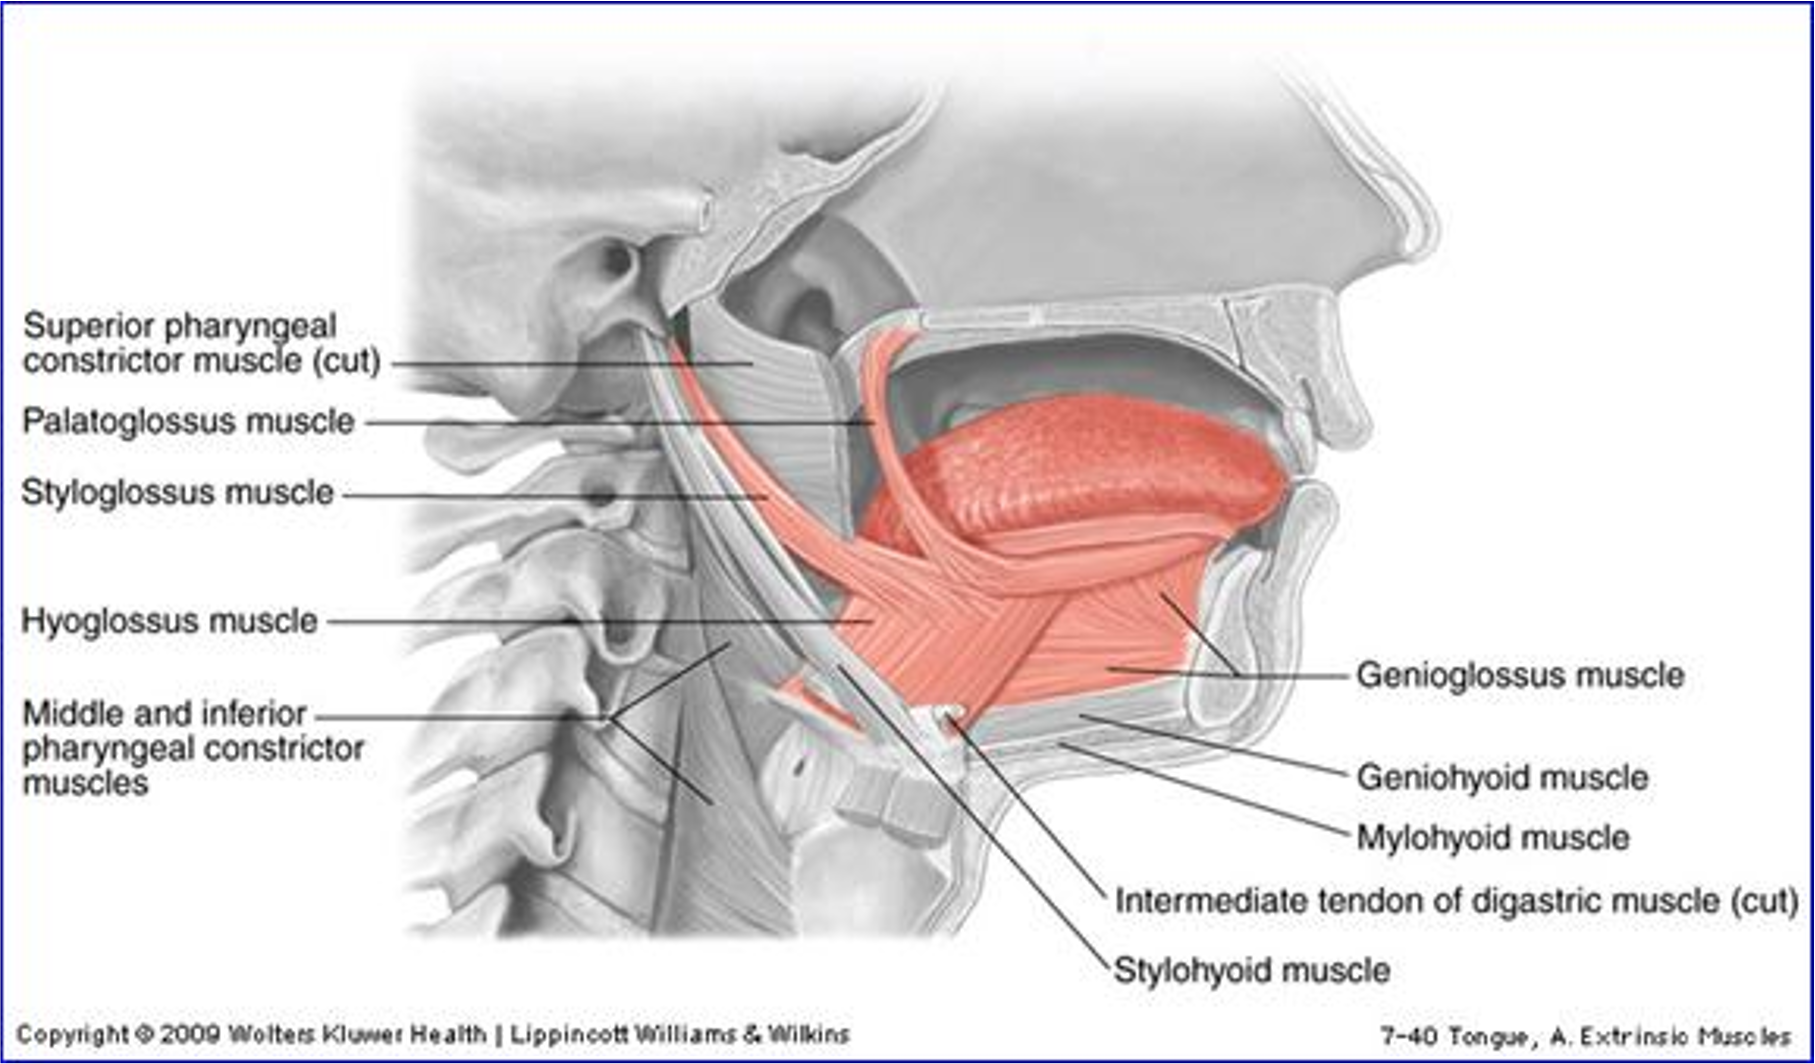
\includegraphics[width = \linewidth]{figs/Tongue.png}
        \columnbreak
        \begin{itemize}
            \item The most widely used articulator
            \item Active for all vowels and most consonants
            \item A muscle anchored to the jaw (by the hyoid bone)
            \item Capable of considerable freedom of movement—especially the anterior (front) part
        \end{itemize}
    \end{multicols}
\end{frame}

\begin{frame}{Major parts of the tongue}
    \begin{itemize}
        \item \textbf{Corona (Front)} – if you stuck your tongue out and put a little paper crown on it, the crown would sit on the coronal parts of the tongue
        \begin{itemize}
            \item \textbf{Tip / apex}
            \item \textbf{Blade} – the part near the front immediately behind the tip
        \end{itemize}
        \item \textbf{Dorsum (Rear)} – think dorsal fin on a dolphin’s back
        \begin{itemize}
            \item \textbf{Center}
            \item \textbf{Back}
        \end{itemize}
        \item \textbf{Root / radix}
    \end{itemize}
\end{frame}

\begin{frame}
    \frametitle{Passive articulators}

    \begin{itemize}
        \item If the tongue is the active articulator for most sounds, what are the passive articulators?
    \end{itemize}
\end{frame}

\begin{frame}
    \frametitle{Passive articulators}

    \begin{center}
        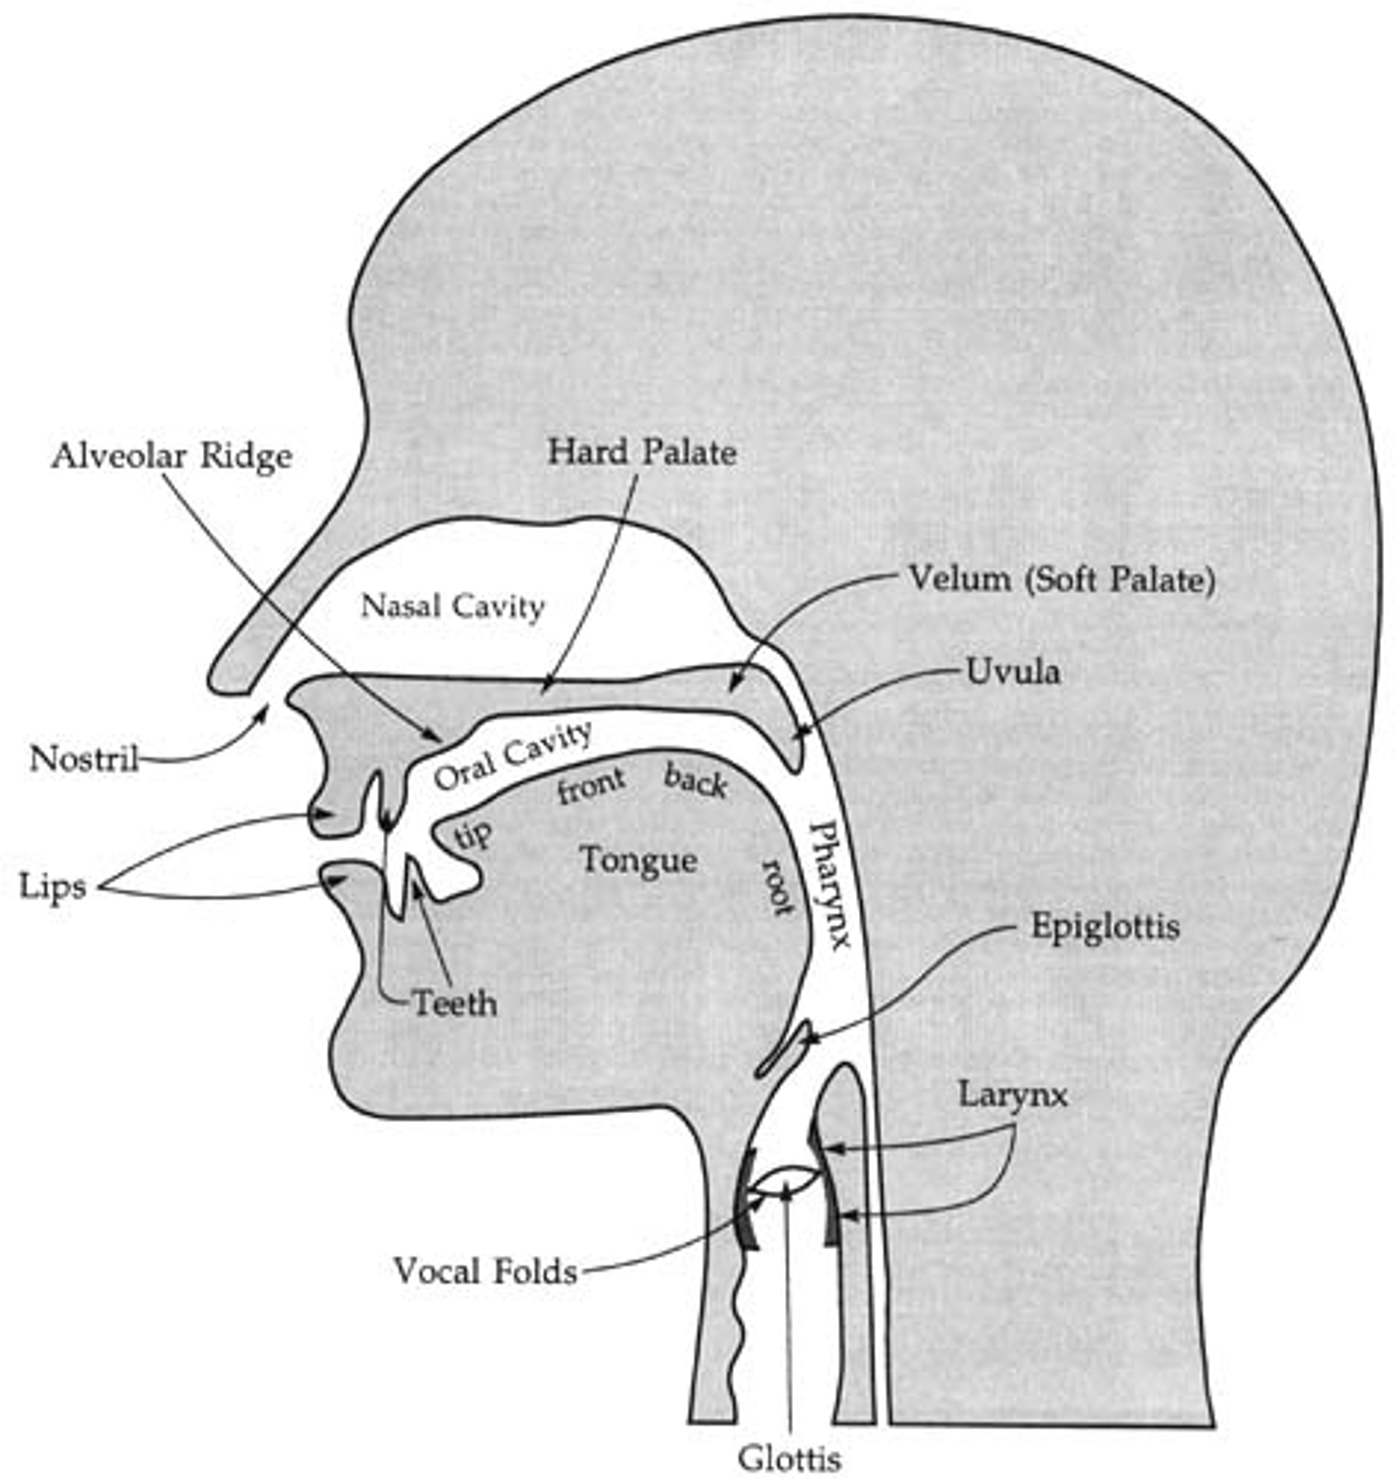
\includegraphics[width = .5\textwidth]{figs/VocalTractLabeled.png}
    \end{center}
\end{frame}

\begin{frame}{The lips}
    \begin{center}
        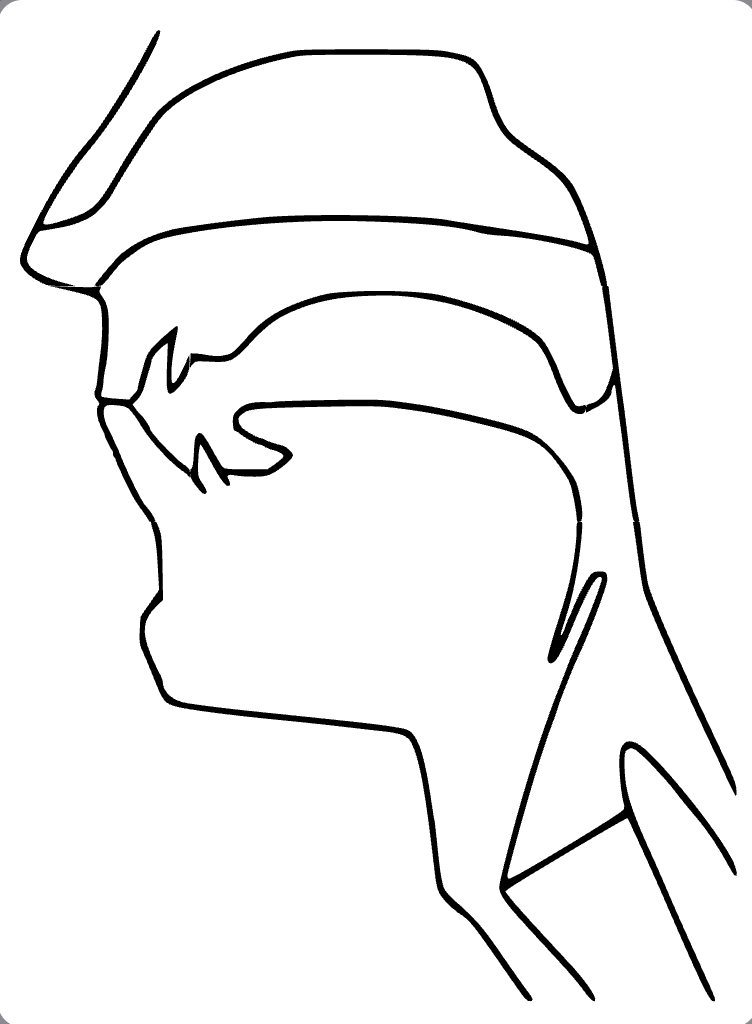
\includegraphics[width = .5\textwidth]{figs/Labials.png}
    \end{center}
\end{frame}

\begin{frame}{The lips}
    \begin{itemize}
        \item Sounds made with the lips are called \textbf{labial}
        \item Sounds where the lower lip touches the upper teeth are \textbf{labio-dental}
        \item Minor point: sounds made with the outer, external part of the lips are exo-labial, those with the inner lip are endo-labial 
    \end{itemize}
\end{frame}

\begin{frame}{Lip Movements}
    \begin{itemize}
        \item \textbf{Rounding} – the lips compress at the corners and squeeze inward
        \item \textbf{Spreading} – the lips straighten and the corners spread (like a smile)
        \item \textbf{Constricting} – the lips block airflow, either somewhat or completely    
    \end{itemize}
    \end{frame}

\begin{frame}{The teeth}
    \begin{center}
        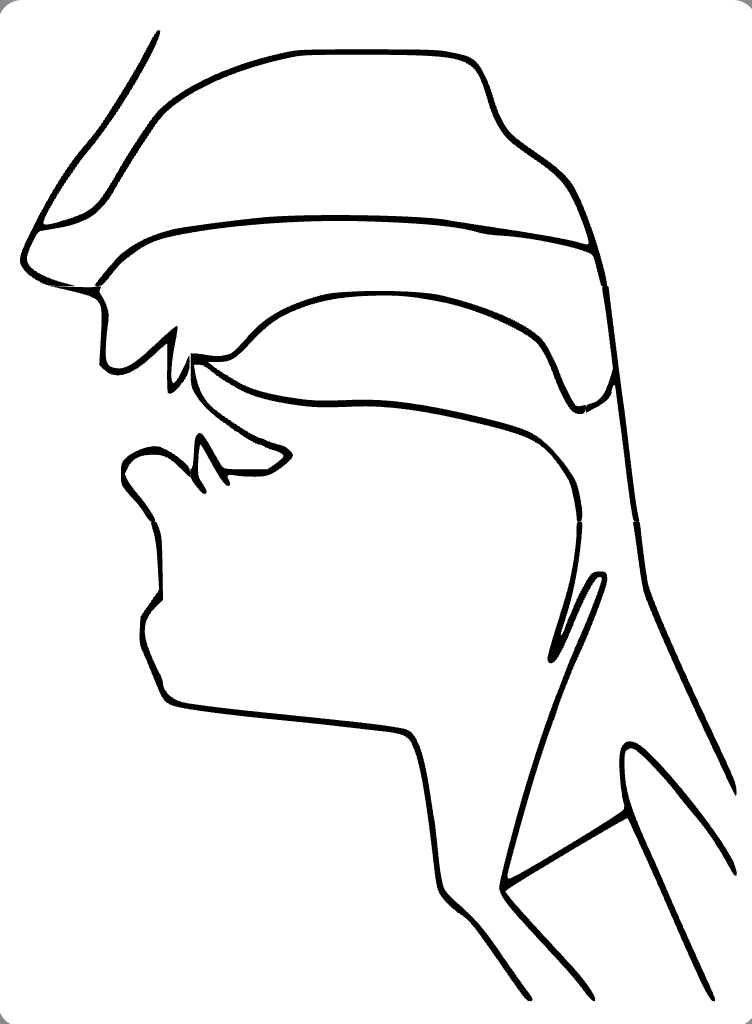
\includegraphics[width = .5\textwidth]{figs/Dentals.png}
    \end{center}
\end{frame}

\begin{frame}{The teeth}
    \begin{itemize}
        \item Incisors and canines are the primary articulators
        \begin{itemize}
            \item Obligatory passive articulators
            \item Only the upper teeth are considered articulators
        \end{itemize}
        \item Sounds made at the teeth are \textbf{dental}
            \item Have acoustic consequences for certain sounds made at other places (especially the sibilant fricatives, we'll talk about this in a few weeks)
    \end{itemize}
\end{frame}

\begin{frame}{The alveolar ridge}
    \begin{center}
        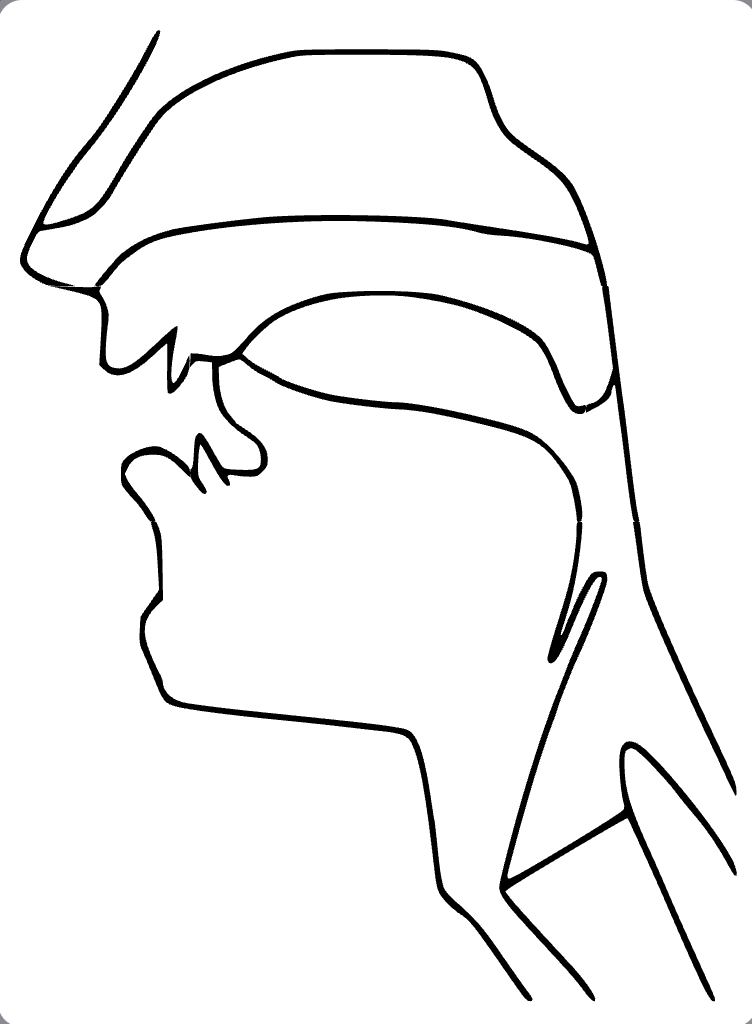
\includegraphics[width = .5\textwidth]{figs/Alveolars.png}
    \end{center}
\end{frame}

\begin{frame}{The alveolar ridge}
    \begin{itemize}
        \item Ridge between the upper teeth and the hard palate
        \item The location of the sockets (alveoli) for the roots of the upper teeth
        \item Not everyone has a clearly defined ridge; some don’t and still talk fine!
        \item Sounds made here are \textbf{alveolar}
        \item Very important place of articulation—the most flexible, nimble part of the tongue can easily make contact here
    \end{itemize}
\end{frame}

\begin{frame}{The palatal}
    \begin{center}
        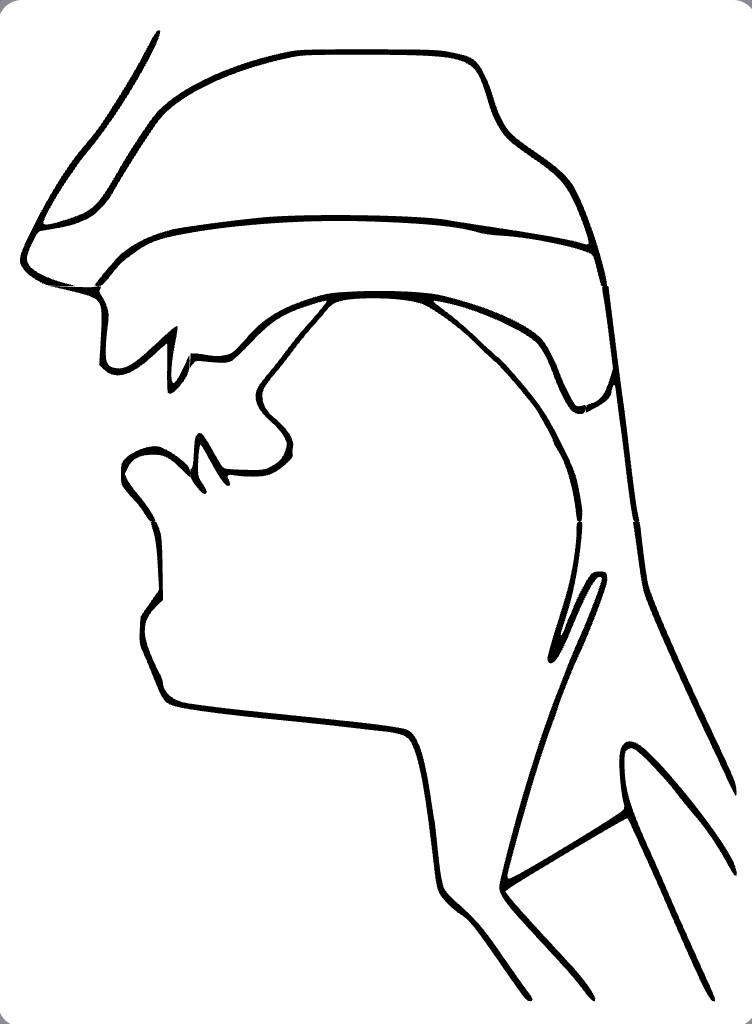
\includegraphics[width = .5\textwidth]{figs/Palatals.png}
    \end{center}
\end{frame}

\begin{frame}{The palate}
    \begin{itemize}
        \item Hard, bony structure; the “roof of the mouth”
        \item Some people have a relatively domed palate, others flatter
        \item Sounds made here are \textbf{palatals}
    \end{itemize}
\end{frame}

\begin{frame}{The velum}
    \begin{center}
        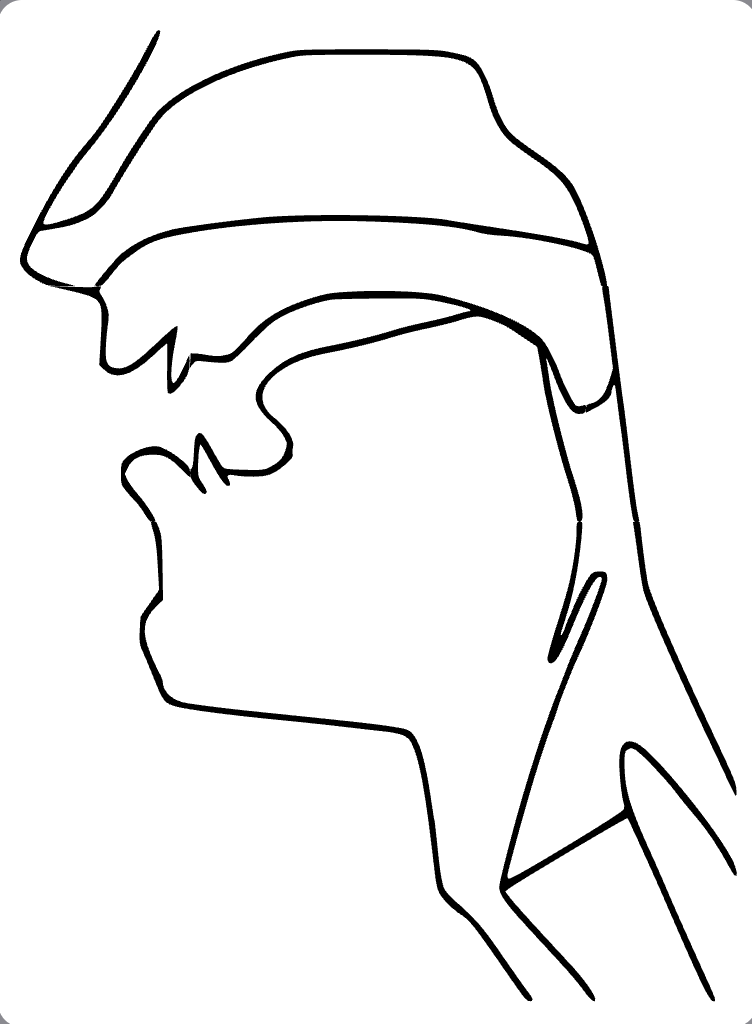
\includegraphics[width = .5\textwidth]{figs/Velars.png}
    \end{center}
\end{frame}

\begin{frame}{The velum}
    \begin{itemize}
        \item Soft tissue (aka the \textbf{soft palate})
        \item As an active articulator:
        \begin{itemize}
            \item Controls the opening of the velo-pharyngeal port (the connection between the oro-pharynx and the nasal cavity)
            \item Allows airflow through the nose for \textbf{nasal} sounds
        \end{itemize}
        \item As a passive articulator:
        \begin{itemize}
            \item Holds still while constriction is actively made by the tongue dorsum
            \item Consonants produced this way are called \textbf{velar}
        \end{itemize}
    \end{itemize}
\end{frame}

\begin{frame}{The uvular}
    \begin{center}
        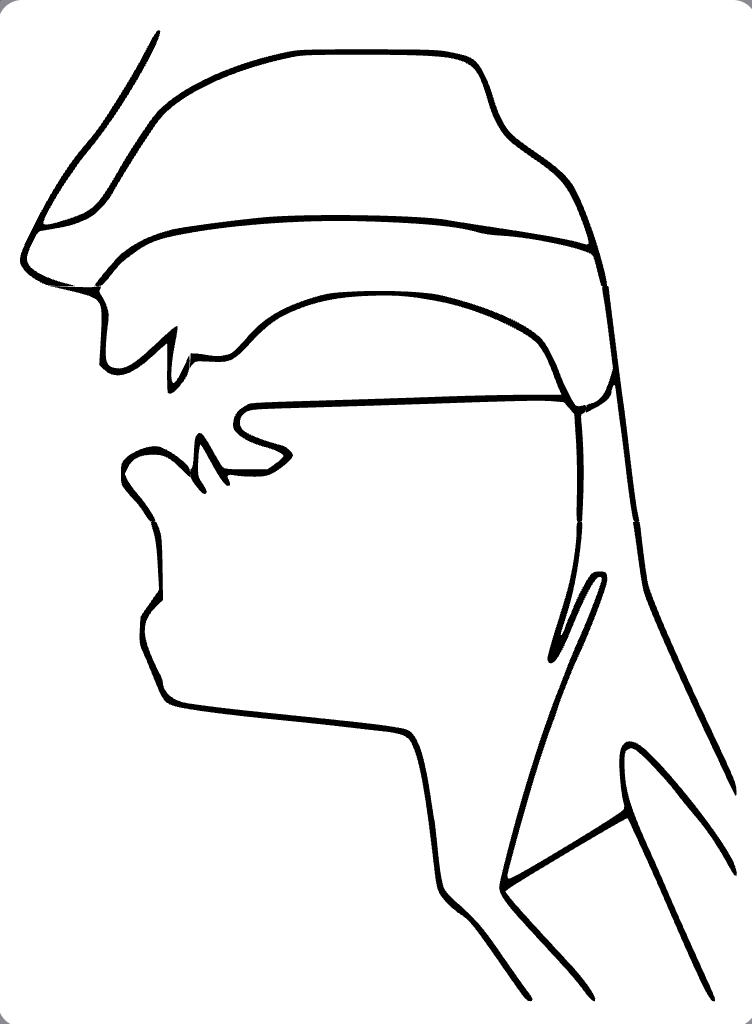
\includegraphics[width = .5\textwidth]{figs/Uvular.png}
    \end{center}
\end{frame}

\begin{frame}{The uvula}
    \begin{itemize}
        \item A fleshy conical extension of the soft palate
        \begin{itemize}
            \item Can be seen if you open your mouth wide and look in a mirror
            \item Fun fact: uvula is Latin for “little grape”
        \end{itemize}
        \item Mainly a passive articulator
        \begin{itemize}
            \item The tongue back moves up and back
            \item Sounds made here are called \textbf{uvular}
        \end{itemize}
        \item As a quasi-active articulator, airflow can be used to vibrate it (uvular trill)
    \end{itemize}
\end{frame}

\begin{frame}{The pharynx}
    \begin{itemize}
        \item The part of the vocal tract below the uvula and above the epi(glottis)
        \begin{itemize}
            \item \textbf{Oral cavity}: cavity between the lips and uvula
            \item \textbf{Oropharynx / buccal cavity}: oral cavity + pharynx
            \item \textbf{Nasopharynx}: pharynx + posterior part of the nasal cavity
            \item \textbf{Throat}: pharynx + glottis + esophagus + trachea
        \end{itemize}
        \item The tongue root can move back towards the pharynx
        \item Sounds made here are \textbf{pharyngeal}
    \end{itemize}
\end{frame}

\begin{frame}{Summary of articulators and adjectives}

    \begin{center}
        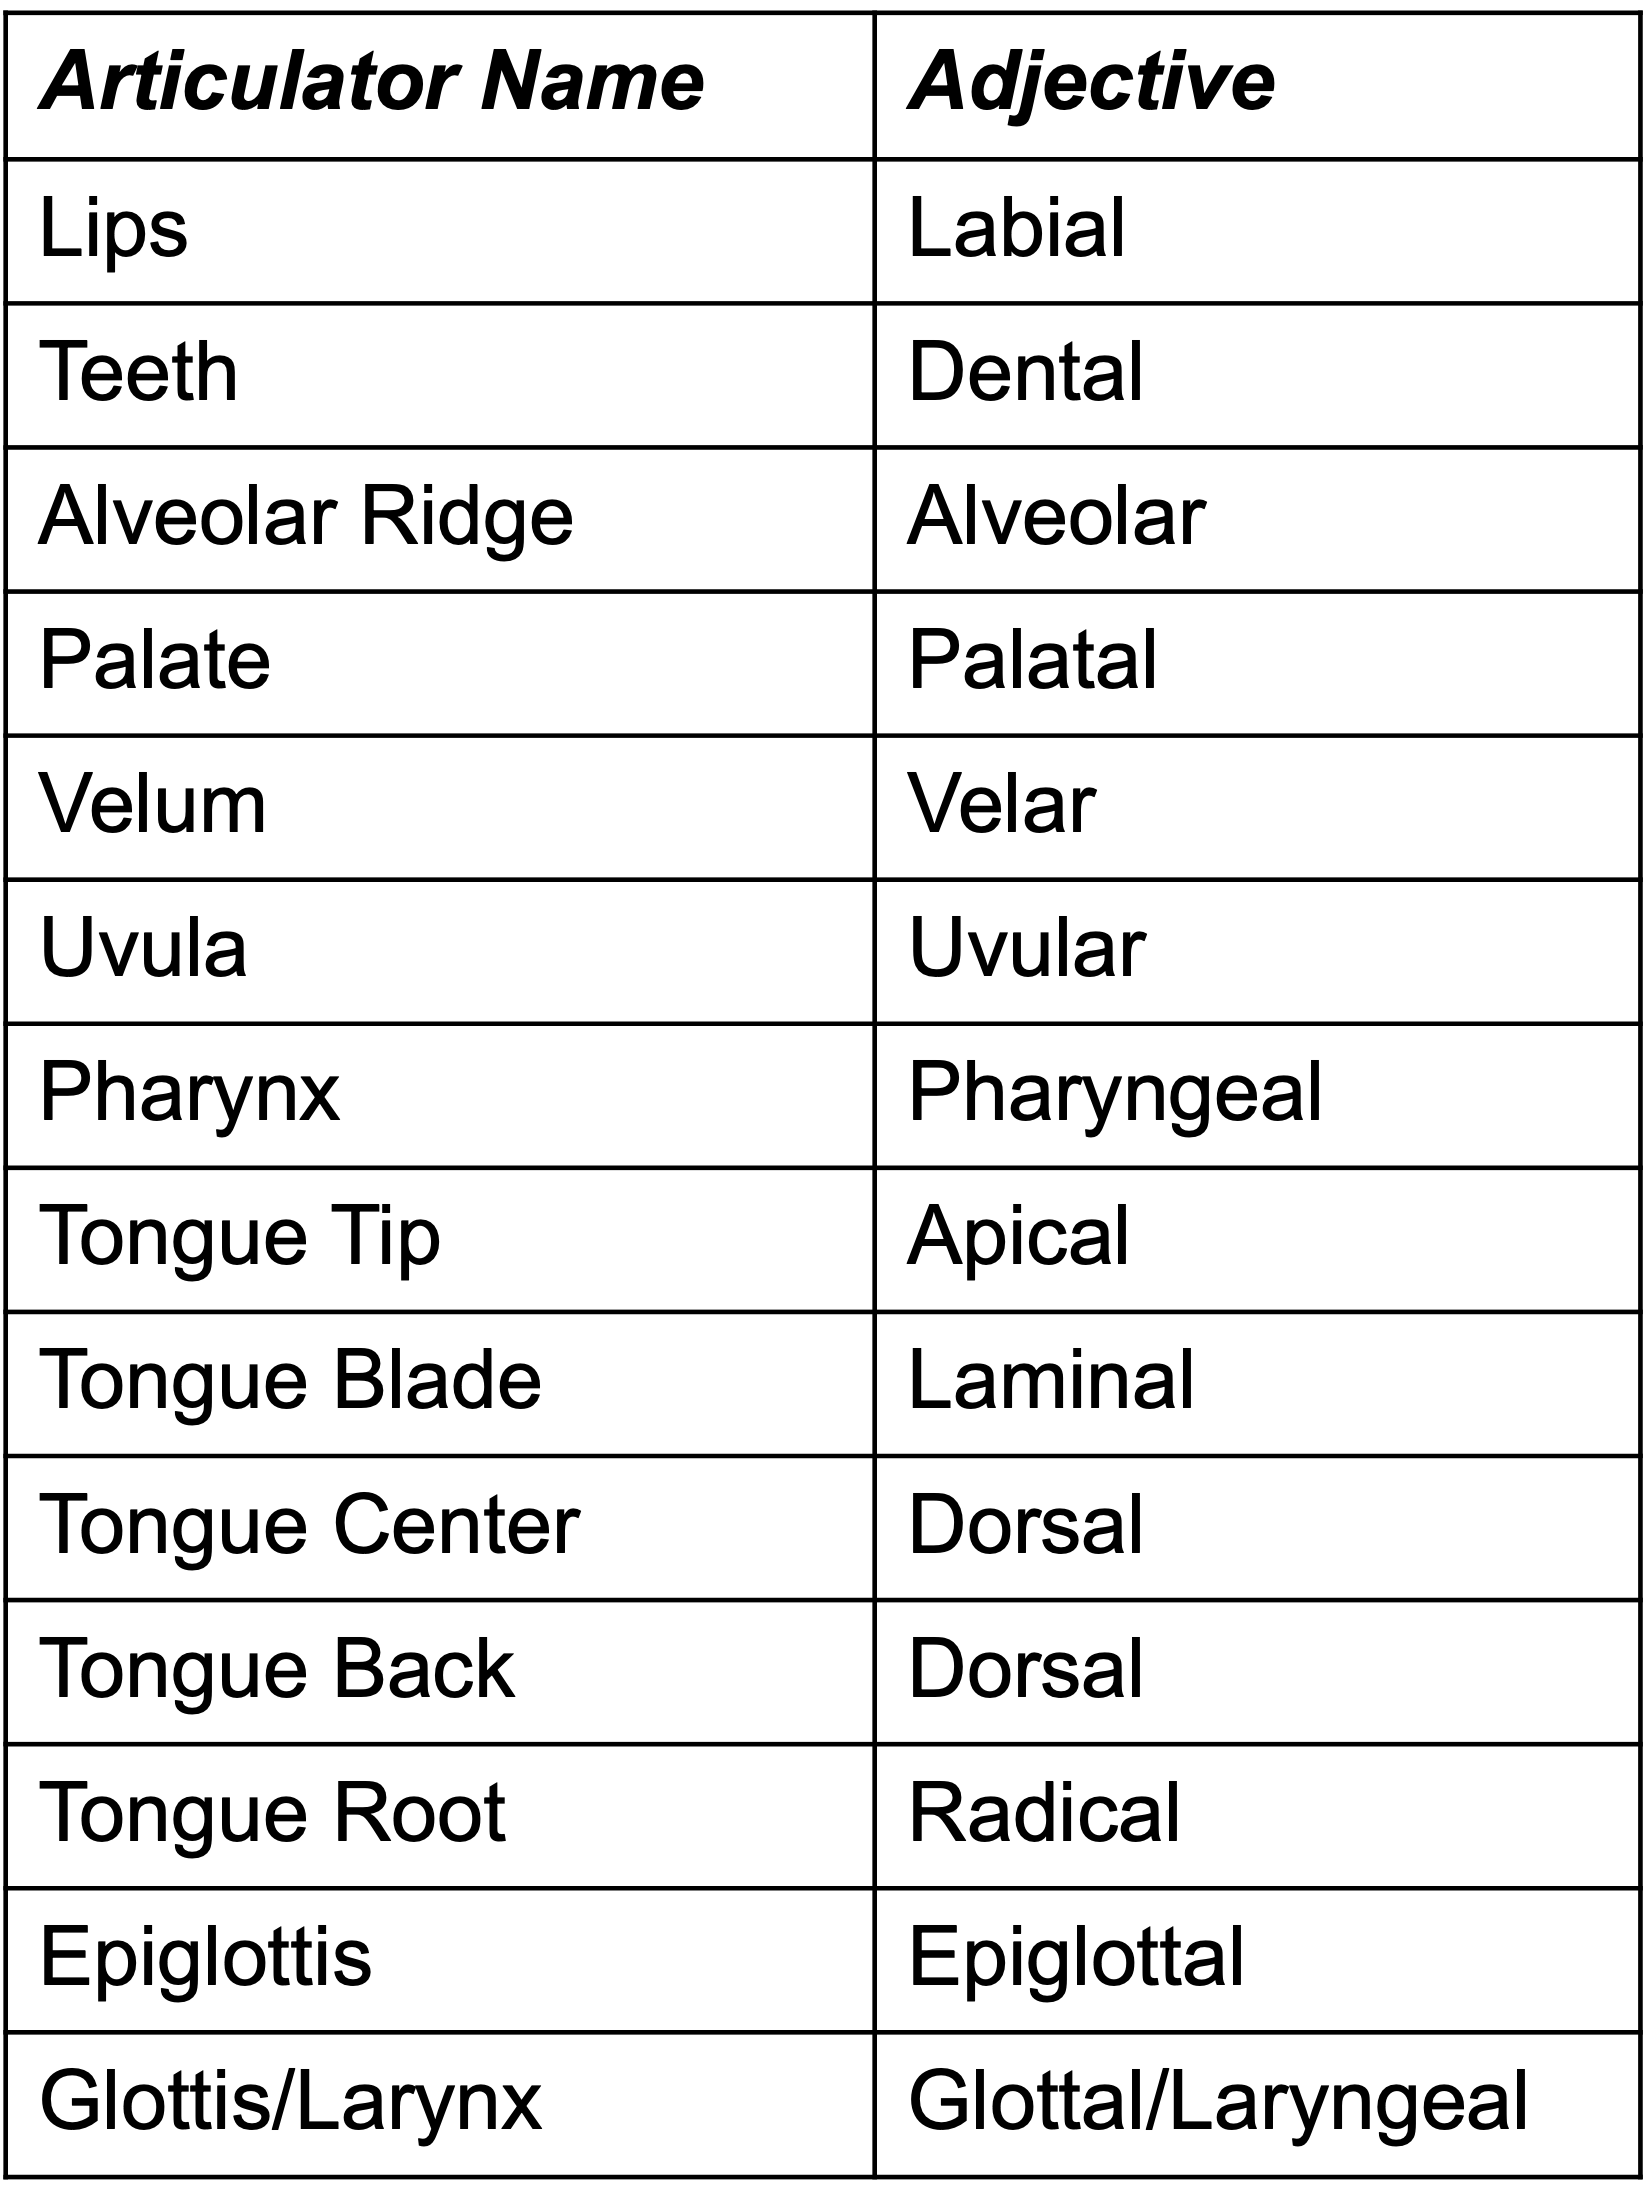
\includegraphics[width = 0.45\linewidth]{figs/Terminology.png}
    \end{center}

\end{frame}

%-----------------------------------------------------------
\section*{To Do:}
%-----------------------------------------------------------
\begin{frame}{To Do:}
    \begin{itemize}
        \item Complete the exit ticket for today on Canvas by 12:30pm.
        \item Complete Homework 2 by Tuesday at 8:30am.
    \end{itemize}
\end{frame}

% \subsection<presentation>*{References}
% %-----------------------------------------------------------
% \begin{frame}[t,allowframebreaks]
%   \frametitle<presentation>{References}
%     \printbibliography
% \end{frame}

\end{document}